\documentclass[11pt, a4paper]{article} % , draft
\usepackage[utf8]{inputenc}

\usepackage{enumitem} % customiçe item dots etc
\usepackage{textgreek} % obv
\usepackage{physics} % for easy derivative notation
\usepackage{amsmath}
\usepackage{amsthm} %theorems
\usepackage{amssymb}
\usepackage{mathtools} % for matrices with blocks inside
\usepackage[scr=boondoxo]{mathalfa}
\usepackage{pst-node}%
\usepackage{mathrsfs}
\DeclareMathAlphabet{\mathpzc}{OT1}{pzc}{m}{it}

\newcommand{\mc}{\multicolumn{1}{c}}
\newcommand{\R}{\mathbb{R}} % command for real R
\newcommand{\Holo}{\mathcal{H}}
\newcommand{\M}{\mathcal{M}}
\newcommand{\C}{\mathbb{C}}
\newcommand{\N}{\mathbb{N}}
\newcommand{\z}{\mathpzc{s}}
\newcommand{\p}{\mathpzc{r}}
\newcommand{\s}{\mathbb{S}}
\newcommand{\W}{\mathbb{W}}
\newcommand{\U}{\mathscr{U}}
\newcommand{\Lg}{\mathscr{L}}
\newcommand{\x}{\mathcal{X}}
\newcommand{\B}{\mathfrak{B}}

\usepackage{csquotes}
\MakeOuterQuote{"}
\setlength{\parskip}{0.3 cm}
\setlength{\parindent}{0 cm}


\usepackage{fancyhdr}

%\usepackage{nath} % authomatic parenthesis stuff
%\delimgrowth=1
\usepackage[left=2cm, right=2cm, top=2.1cm, bottom=2.1cm]{geometry} % set custom margins
\usepackage{graphicx} % to insert figures
\usepackage{grffile}
\graphicspath{{Figures/}} % define the figure folder path
\usepackage{subcaption} % for multiple figures at once each with a caption
\usepackage{multirow} %multirow in tables

\usepackage{caption}
\captionsetup[figure]{font=footnotesize} %adjust caption size
\captionsetup[table]{font=footnotesize} %adjust caption size

\usepackage{booktabs} % for pretty tabs in tables
\usepackage{siunitx} % Required for alignment
\captionsetup{labelfont=bf} % bold face captations

\usepackage{hyperref} % makes every reference a hyperlink
\hypersetup{
    colorlinks=true,
    linkcolor=violet,
    filecolor=[rgb]{0.69, 0.19, 0.38},      
    urlcolor=[rgb]{0.0, 0.81, 0.82},
    citecolor=[rgb]{0.69, 0.19, 0.38}
}

\usepackage{epigraph} % for quotations in teh begginig
\setlength\epigraphwidth{8cm}
\setlength\epigraphrule{0pt}
\usepackage{etoolbox}
\makeatletter
\patchcmd{\epigraph}{\@epitext{#1}}{\itshape\@epitext{#1}}{}{}
\renewcommand{\qedsymbol}{o.\textepsilon.\textdelta}

\newtheorem{prop}{Proposition} %so I can use propositions
\newtheorem{cor}{Corollary} %so I can use corollaries
\newtheorem{defi}{Definition} %so I can use corollaries

\makeatother % all this is for the epigraph
\usepackage{tocloft}

\usepackage{imakeidx} % make index

\makeindex[columns=3, title=Alphabetical Index, intoc]

%\title{\vspace{-2.5cm} {\bf Can we make the Exponential scaling in Time\\ be Linear in Time if Parallelized Exponentially? \\ {\em - Part 2 -}} \vspace{-0.4cm}  }
\title{\vspace{-2cm} {\bf Reality and Causality in the Microscopic World:\\ A Discussion from Quantum Transport Theories}%\\{\small by {\em Xabier Oyanguren Asua}}
\vspace{-0.4cm}}
\date{\vspace{-11ex}}
\let\clipbox\relax
\usepackage{adjustbox}
\newcolumntype{?}{!{\vrule width 1.5pt}}
\usepackage{abstract}
\setlength{\absleftindent}{0mm}
\setlength{\absrightindent}{0mm}

\usepackage{tcolorbox}
\DeclareRobustCommand{\mybox}[2][gray!10]{%
\begin{tcolorbox}[   %% Adjust the following parameters at will.
        left=0.2cm,
        right=0.2cm,
        top=0.15cm,
        bottom=0.15cm,
        colback=#1,
        colframe=#1,
        width=\dimexpr\textwidth\relax, 
        enlarge left by=0mm,
        boxsep=5pt,
        arc=0pt,outer arc=0pt,
        ]
        #2
\end{tcolorbox}
}

\usepackage{anyfontsize}
\newenvironment{kapituloBerria}[1][]
  {\clearpage           % we want a new page          %% I commented this
   \thispagestyle{empty}% no header and footer
   \vspace*{\stretch{2}}% some space at the top
   \raggedleft          % flush to the right margin
   {\textbf{{\fontsize{60}{40}\selectfont \hspace{+9.5cm}#1\newline \newline}}}
   \bf
   \fontsize{30}{20}\selectfont
  }
  {\par % end the paragraph
   \vspace{\stretch{3}} % space at bottom is three times that at the top
   \clearpage           % finish off the page
  }

\usepackage{listings}
\usepackage{xcolor}
\lstset{language=C++,
                basicstyle=\ttfamily,
                keywordstyle=\color{blue}\ttfamily,
                stringstyle=\color{red}\ttfamily,
                commentstyle=\color{green}\ttfamily,
                morecomment=[l][\color{magenta}]{\#}
    backgroundcolor=\color{black!5}, % set backgroundcolor
    basicstyle=\footnotesize,% basic font setting
}
%\DeclareMathSizes{display size}{text size}{script size}{scriptscript size}.
\DeclareMathSizes{10}{10}{10}{10}
\setlength{\footnotesep}{0.55\baselineskip}
\begin{document}
\pagenumbering{gobble}



\maketitle



{\bf Chapter on {\em “Physics and the Nature of Reality: Essays in Memory of Detlef Dürr”.}}

\begin{center}
{\bf Abstract }
\end{center}
Paraphrasing Feynmann, perhaps, the main reason why the so-called Copenhagen (or orthodox) quantum theory is so popular among the physicists and engineers is because “I can safely say that nobody understands [it]”. Many physicists and engineers take profit of the mathematical machinery of the Copenhagen theory without paying attention to its ontology, which implies that a quantum object has no microscopic properties (unless a property is measured, or the quantum object is an eigenstate of some property). Such an orthodox view of a microscopic world, empty of properties, is specially unsuitable to understand and to develop approaches to predict modern nanoelectronics, as we discuss along this chapter. As an alternative, physicists dealing with the foundations of quantum transport and open systems have developed different approaches in terms of some type of causal motion of electrons. When dealing with nanodevices, the Copenhagen ontology affirms that electrons are nowhere since their positions are undefined until measured, while causal motion approaches say that electrons can be perfectly understood as particles traversing a device with well-defined positions, independently of the measurement. This last view certainly holds true for treatments based on the Bohmian theory. Even for quantum phenomena of light, such as spontaneous emission or photon partition noise, the Bohmian theory allows an explanation from well-defined electromagnetic fields interacting with electrons, which is contrary to the standard Copenhagen approach. The above examples, developed in this chapter, emphasize that the main merit of the Bohmian theory is eliminating the observer/measurement as the “creator” of the microscopic reality, showing that a well-defined description at all times, of the microscopic properties of a quantum system, is available (where particles are particles and fields are fields at all times). Such a microscopic description does not only provide conceptual advantages, but also important numerical ones when electron devices are understood, in general, as non-Markovian open quantum systems.   

\newpage
\pagenumbering{arabic}
\setcounter{page}{1}
\begin{center}
\section*{ Bohmian Mechanics as a Practical Tool:\\ \vspace{0.2cm} \small when tools harnessing beyond-observable notions happen to be Bohmian in disguise }\vspace{-0.4cm}
{\bf \small - Chapter on {\em “Physics and the Nature of Reality: Essays in Memory of Detlef Dürr” - }}\vspace{-0.32cm}
\end{center}

\hspace*{4mm} In front of the incapacity of the standard quantum theory (so called orthodox interpretation), to answer "when", "for how long" or whether "there are" electrons crossing the transistors of our phones at all, any physicist or engineer that needs to consider that this is indeed the case for the practical development of cutting edge devices, resorts to alternative explanations of quantum phenomena in terms of electrons that actually do cross their transistors \cite{where}. The well known Bohmian explanation is one such alternative to the orthodox interpretation \cite{Bohm,Holland, Durr,JordiXavier}. \vspace{-0.1cm}

Wondering if there are electrons in our phones sounds like a rhetorical joke, and yet, technically, the orthodox quantum theory is not able to affirm it. Under this theory, a quantum system {\bf has} a property only when its wavefunction is an eigenstate of the associated operator. This can only be assured if it is strongly measured. Consequently, it is meaningless to talk about properties of the electrons in the active regions of nanoscale devices, since while in operation, they are not being strongly measured and they might be in an arbitrary superposition of eigenstates  \cite{where}. If anything, it is an environment portion entangled with these oscillating electrons that is being strongly measured (say, the cable connected to the active region); not the nanometric active region itself. Thus, the "reality" of any property for the electrons within it, even their position, is unacceptable for the standard theory. And yet, no engineer can seriously believe that there is no electron in an operating nano-device like a transistor.\vspace{-0.1cm} %In its terms, it is still obscure something as fundamental for modern electronics as the quantum treatment of nanoscale devices operating at high frequencies \cite{Thz}.

More importantly however, even if one turns a blind eye to these "technical unspeakability" considerations, for which the true orthodox voluntarily hold their tongues, their tool-set is itself limited as well. Under the restriction of these tools, the modeling of some scenarios looks unnecessarily pathological, leaving tied the hands of the orthodox, in addition to their tongues. Example of such {\bf practical} limitations of the standard theory are the "difficulty" in the search of an operator for the multi-electron displacement current \cite{equiv, Pel} or the "cumbersome" demand of a high frequency measuring apparatus to be simulated as a non-Markovian environment \cite{Thz}. As ironic as it is, the orthodox that even still look for tools that allow the prediction of the phenomenological manifestations of such "pathological" scenarios (to predict the expectation or correlation of dynamical variables or predict the reduced density of non-Markovian open quantum systems), "accidentally" resort to concepts like weak measurements or the conditional wavefunction, which are Bohmian in disguise, as we will explain \cite{interpretSSE,NMisModal}.\vspace{-0.1cm}

In this chapter, we will take a trip around several hot-spots where Bohmian mechanics and its capacity to describe properties in the absence of strong measurements are being harnessed as computational tools, in order to get phenomenologically accessible information. We will then justify how the additional step to assume an ontological interpretation for such pragmatic tools, turns out to be practically useful, even when one is only interested in the orthodox variables.

% As we will discuss along the chapter, satisfying and practically useful explanations for these, apparently seem to demand the use of modal theories like Bohmian mechanics. 

We can easily arrive to these conclusions through the concepts of conditional wave-function (CWF) and effective wave-function (EWF), introduced by {\em Dürr et al.} in Ref. \cite{Absolute}, together with the understanding of the measurement dilemma they enlighten. We will therefore review them in the first section, along with how the density matrix formalism and any general quantum operation can be understood in such Bohmian terms. These will lead us in a natural way to the main theses of the chapter. For instance in section two, we will show how a Stochastic Schrödinger Equation (SSE), used to compute the reduced density matrix of a non-Markovian open quantum system, necessarily seems to employ CWF-s. We will see that by dressing these CWF-s with an interpretation, the Bohmian theory can prove to be a useful tool in the search for SSE-s. In section three, we will introduce how any orthodox observable (except perhaps the spin) can be computed from Bohmian trajectories, as if it was a property of each trajectory, so conveniently as to even be able to derive the observable operator itself. On the "unspeakables", since the Bohmian trajectory of an "unmeasured" system is defined at all times, we will be able to speak about its defined properties in a compatible way with phenomenology. What is more, we will see that in fact those "unmeasured" system properties can indeed be measured, which will bring about several practical applications.


%Let us first shortly review this, to then find three applications in nano-electronics, that prove the practical usability of all the Bohmian theoretical framework.

\subsection*{1. The Reach of the Bohmian Narrative: A Suggestive Review}
\vspace{-0.2cm}

\subsubsection*{1.1. The Conditional and Effective Wavefunctions}
\vspace{-0.2cm}

Given a quantum system of $N$ degrees of freedom described by the real coordinate vector $\vec{q}=(q_1,..., q_n)\in\Omega_t\subseteq\R^N$, we can describe its evolution in continuous time $t\in\R$, with the use of a complex wavefunction $\Psi(\vec{q},t)=\rho^{1/2}(\vec{q},t)e^{i\mathcal{S}(\vec{q},t)/\hbar}$ (encoding the two real fields $\mathcal{S}$ and $\rho$), and an associated Bohmian trajectory $\vec{q}^{\:\xi}(t)\equiv \vec{q}\:(\vec{\xi},t)$ the initial condition of which is given by the label space vector $\vec{\xi}\in\Omega_0\subseteq\R^N$ such that $\vec{q}^{\:\xi}(t=0)=\vec{\xi}$. This trajectory is guided by the wavefunction through the "guidance law", while the wavefunction itself is guided by the Schrödinger Equation \cite{Bohm,Holland,Durr,JordiXavier}. Respectively:\vspace{-0.2cm}
\begin{equation}\label{GL}
\dv{q_k^{ (\xi)}(t)}{t} = v_k(\vec{q},t)\Big\rvert_{\vec{X}=\vec{q}^{\:\xi}(t)}:=\frac{1}{m_k} \pdv{\mathcal{S}(\vec{q},t)}{x_k}\Big\rvert_{\vec{q}=\vec{q}^{\:\xi}(t)}
\end{equation}
\begin{equation}\label{SE}
i\hbar\pdv{\Psi(\vec{q},t)}{t}=\Big[ \sum_{k=1}^N \frac{\hbar^2}{2m_k}\pdv[2]{}{q_k}+U(\vec{q})\Big]\Psi(\vec{q},t)
\end{equation}
where $m_k$ is the mass associated with the $k$-th degree of freedom, $v_k$ is the velocity field piloting the $k$-th degree of the Bohmian trajectories and $U$ denotes the classical potential describing the interaction between the degrees of freedom (since we consider an isolated system we assume no time dependence, but we could describe in general a closed system by allowing it to vary in time). The most general isolated system we could consider is the whole Universe, where $\vec{q}$ would reflect its degrees of freedom or {\bf configuration}. Then, by the quantum equilibrium hypothesis \cite{Absolute}, our Universe has the trajectory labeled by $\vec{\xi}$ with a probability density function $|\Psi(\vec{q}\,(\vec{\xi},t),t)|^2$ (squared magnitude). 

Let us now partition the whole Universe in a subsystem of interest S, of $n<N$ degrees of freedom $\vec{x}=(x_1,...,x_n)$, and its environment, of degrees of freedom $\vec{y}=(y_{n+1},...,y_N)$; where we identify $\vec{q}\equiv (\vec{x},\vec{y})$. We could associate one wavefunction to the system and one to the environment, both labeled by the initial joint configuration $\vec{\xi}$, as $\psi^\xi(\vec{x},t):=\Psi(\vec{x},\vec{y}^{\:\xi}(t),t)$ and $\phi^\xi(\vec{y},t):=\Psi(\vec{x}^{\:\xi}(t),\vec{y},t)$. These are particular cases of the so called {\bf conditional wavefunctions} (CWF-s). In general, a CWF is a slice of a wavefunction, obtained by evaluating some of its degrees of freedom along a (Bohmian) trajectory, while leaving the rest un-evaluated \cite{Absolute, JordiXavier}. As such, note that given the positions of the evaluated degrees of freedom, the "conditional" probability density for the rest of the system will be given by the squared magnitude of the CWF, since for instance $|\Psi(\vec{x},\vec{y}^{\:\xi}(t), t)|^2=|\psi^\xi(\vec{x},t)|^2$.

As proved in \cite{GJ}, the full Schrödinger Equation \eqref{SE}, ruling the dynamics of the whole, can be re-written exactly into two coupled dynamical sets of equations ruling the motion of the two presented CWF-s. For the system we have\footnote{For the environment they will be the same but changing the CWF and the index ranges.}:\vspace{-0.2cm}
\begin{equation}\label{SE.GJ}
i \hbar \pdv{\psi^\xi (\vec{x},t)}{t} = \qty[\sum_{k=1}^n\frac{\hbar^2}{2m_k} \pdv[2]{}{x_k} +  U(\vec{x}, \vec{y}^{\: \xi}(t)) + G(\vec{x}, \vec{y}^{\: \xi}(t),t)+i\ J(\vec{x}, \vec{y}^{\: \xi}(t),t)] \psi^\xi (\vec{x},t)
\end{equation}
with $G$ and $J$ the real and complex parts of the so called {\bf quantum correlation potential}:
\begin{equation}\label{G.Bohm}
G(\vec{x},\vec{y}^{\:\xi}(t),t):=\sum_{j=n+1}^N\qty[-\frac{1}{2}m_j\qty(v_j(\vec{x},\vec{y}^{\: \xi}(t),t))^2-\frac{\hbar^2}{2m_j\rho^{1/2}(\vec{x},\vec{y}^{\:\xi}(t),t)}\qty(\pdv[2]{\rho^{1/2}(\vec{x},\vec{y},t)}{y_j})\Big\rvert_{\vec{y}=\vec{y}^{\:\xi}(t)} ]\vspace{-0.2cm}
\end{equation}
\begin{equation}\label{J.Bohm}
J(\vec{x},\vec{y}^{\:\xi}(t),t):=-\frac{\hbar}{2}\sum_{j=n+1}^N\pdv{}{y_j}v_j(\vec{x},\vec{y},t)\Big\rvert_{\vec{y}^{\, \xi}(t)}
\end{equation}
where we recognize as $G$ the difference between the quantum potential \cite{JordiXavier, Durr} and the kinetic energies of the trajectory of the environment, and as $J$, the spatial variation in the environment axes $y_j$ of their associated Bohmian velocity. All these are terms that involve a derivative of the phase $\mathcal{S}$ or the magnitude $\rho$ of the full wavefunction $\Psi$ in the environment coordinates $\vec{y}$ centered at the trajectory position $\vec{y}^{\:\xi}(t)$. This means that in order to compute them, we would not have enough with the two slices $\psi^\xi(\vec{x},t)$ and $\phi^\xi(\vec{y},t)$. We would require the information of the other adjacent CWF-s evaluated in $\vec{y}$ close to but not exactly in $\vec{y}^{\:\xi}(t)$. This is an explicit manifestation of the so called quantum wholeness \cite{JordiXavier}, by which the dynamics of a single Bohmian trajectory depends on the dynamics of the rest of possible trajectories. Thus, we see that while $U$ introduces all the classical correlation between the system and the environment, the responsible ones for their quantum interaction (the interaction with the rest of possible Bohmian trajectories) are $G$ and $J$.\footnote{Note that while multiple stacked CWF-s for the subsystem around $\vec{y}^{\:\xi}(t)$ are required to compute $G$ and $J$, the guidance for the trajectory of the subsystem $\vec{x}^{\:\xi}(t)$, is given entirely by the CWF at $\vec{y}^{\:\xi}(t)$: denoting $\psi^\xi (\vec{x},t)=r^\xi(\vec{x},t)e^{is^\xi(\vec{x},t)/\hbar}$, then $\dv{}{t}x_k^{(\xi)}(t)=\frac{1}{m_k}\pdv{s^\xi(\vec{x},t)}{x_k}\big\rvert_{\vec{x}=\vec{x}^{\:\xi}(t)}$ for $k\in\{1,...,n\}$.}\vspace{-0.15cm}

%The same set of equations for the environment (with the proper changes of indices and CWF), together with these, would yield a description of the dynamics of the whole Universe in two partitions, that are coupled classically through $U$ and quantically through $G$ and $J$.

%It is clear that the time evolution of the two CWF-s is not independent, nor they are independent to the full wavefunction. This is because knowledge of the derivatives of the full wavefunction in the evaluated axes $\vec{y}$, $\pdv{\Psi(\vec{X},t)}{x_k}\Big\rvert_{y^\xi(t)}$ for $k\in\{m+1,...,N\}$, is necessary to compute $G$ and $J$, which means that all the CWF-s $\Psi(\vec{x},\vec{y}^\eta(t),t)$ with $\vec{y}^\eta(t)$ close to $\vec{y}^{\:\xi}(t)$ are required (not just one CWF over the trajectory). This means, that in general the sub-system will evolve differently as a function of the environment trajectory and the full wavefunction's evolution.

Now, the only way in which the subsystem CWF $\psi^\xi(\vec{x},t)$ can behave as if it was an independent closed quantum system wavefunction, ruled by a unitary Schrödinger Equation \eqref{SE} and interacting only classically with its environment (through $U$), is if both $G$ and $J$ vanish.\footnote{ If only $J$ vanished, the CWF would already be ruled by a unitary Schrödinger Equation, with a real potential: $V(\vec{x},t):=U(\vec{x},\vec{y}^{\:\xi}(t))+G(\vec{x},\vec{y}^{\:\xi}(t),t)$. Yet, computationally, a quantum description for the environment in order to evaluate $G$ would still be required, meaning it would not truly be an independent closed quantum system. } Whenever this is the case, we can say that the CWF of the system is its {\bf effective wavefunction} (EWF). The question is then: when are $J$ and $G$ (the quantum influences of the environment on the subsystem) negligible? One of the most important cases in which this happens is after a strong measurement of the subsystem. 


%When the full wavefunction's variation along the axes of the E, $\vec{y}$, in the neighborhood of its trajectory $\vec{y}^{\:\xi}(t)$, is negligible: $\pdv{\Psi(\vec{x},\vec{y},t)}{x_j}\rvert_{\vec{y}=\vec{y}^{\:\xi}(t)}\simeq 0  \quad \forall j\in\{n+1,...,N\}$, both $G$ and $J$ will vanish, as they involve derivatives of the magnitude $\rho^{1/2}$ and the phase $S$ of the wavefunction $\Psi$ in the axes of the E, $\vec{y}$, around $\vec{y}^{\:\xi}(t)$. For example, this is the case when the CWF-s of the S, $\psi^\xi(\vec{x},t)$, are significantly different only if macroscopically distant CWF-s are considered (along $\vec{y}$), or when equal CWF-s of the S are piled in macroscopically distant and disjoint supports in configuration space, as we will see.

%Graphically, this happens for instance when the full wavefunction $\Psi$ is composed of disjoint and macroscopically separated stackings of almost similar CWF-s in $\vec{x}$ \footnote{More quantitatively, the statement "macroscopically far" means that the variation of the (normalized) conditional wavefunction in the $\vec{y}$ axes happens only if a macroscopically big distance is considered. This implies that for any significant time for the subsystem, the evolution of the environment (the dynamics of the wavefunction in the $y$ axes) will not affect the current shape of the CWF in $x$.} (this will be useful to see why countable spectrum projective measurements effectively generate "collapsed" eigenstates). The same can happen as well if the variation of the full wavefunction in $y$ is arbitrarily slower than the variations in $x$ (which will be useful to see why continous measurement schemes generate very narrow gaussians as "collapsed" wavefunctions).
\vspace{-0.2cm}

\subsubsection*{1.2. Measurement understood as unitary evolution using Bohmian CWF-s and EWF-s}
%The concept of CWF and EWF allow a Bohmian explanation of the quantum measurement without the need of any sort of so called "collapse", as formulated by the orthodox explanation to break the von Neumann chain of coupling. This is essential for the following discussion of the chapter, so we will quickly review it as well.
\vspace{-0.1cm}
Given the initially closed quantum system S and its EWF $\psi(\vec{x},t)$, to take a strong measurement of an arbitrary property $B$, as suggested by von Neumann \cite{vonNeumann} and explained in terms of Bohmian mechanics in Refs. \cite{Durr, JordiXavier, Holland}, we can consider the position of the dial of a macroscopic measuring apparatus M. Its generalized coordinate $z\equiv y_{n+1}$ (part of the environment for S), is what is really observed by the experimenter. We prepare the EWF of this dial to be a fiducial state that will make sure its Bohmian position at the first time of the measurement $t=0$, given by $z^{\:(\xi)}(t=0)$, is reliably around the macroscopic rest position of the dial $z=0$, with a high precision and accuracy. For example $\varphi(z,t=0)=c e^{-z^2/4\sigma^2}$, or in ket notation $\ket{\varphi(t=0)}_M=\int\varphi(z,0) \ket{z}dz$,  with $c=1/((2\sigma\pi)^{1/4})$ a normalization constant and $\sigma$ small. We now let S, which in ket notation has state $\ket{\psi(0)}_S=\int\psi(\vec{x},0)\ket{\vec{x}}dx$, interact with the measurement dial M through the von Neumann Hamiltonian $\hat{H}_{MS}=\bar{\mu}(t)\,\hat{p}_M\otimes \hat{B}_S$, where $\hat{p}_M$ is the momentum operator of the dial and $\hat{B}_S$ is the operator related with the property $B$ of the system we wish to measure. $\bar{\mu}(t)$ times the interaction since it has support only in $t\in(0,T)$ (the interaction time) and shows the measurement strength as $\mu:=\int_0^T\bar{\mu}(t)dt$. 

If the observable $B$ has countable spectrum, such that $\hat{B}_S=\sum_k b_k \ket{b_k}_S\bra{b_k}_S$, with $\{\ket{b_k}_S\}_k$ an orthonormal basis of S and $\ket{\psi(0)}_S=\sum_k \beta_k(0)\ket{b_k}_S$: at the last interaction time $t=T$, the unitary Schrödinger evolution $\hat{U} \null_{0}^T=e^{-i\mu T \hat{H}_{MS}/\hbar}$ will leave the composed initial state $\ket{\Phi(0)}_{MS}=\ket{\varphi(0)}_M\otimes\ket{\psi(0)}_S$ as:\vspace{-0.15cm}
\begin{equation}\label{postM1}
\ket{\Phi(T)}_{MS}=\sum_k \beta_k(0)\qty(\int c e^{-\frac{(z-b_k\mu T)^2}{4\sigma^2}}\ket{z}_M dz )\ket{b_k}_S
\end{equation}
This means that if the interaction strength $\mu$ or time $T$ are big enough, or $\sigma$ is small enough, the probability density for the Bohmian position of the dial $z$, is exclusively concentrated in several (roughly) disjoint Gaussians of weights $|\beta_k(0)|^2$ in $z$, each centered in a different $b_k \mu T$ position for $z$, around which, the (normalized) CWF for the system S is $\ket{b_k}_S$ (the eigenstate linked to the eignevalue that locates its envelope Gaussian). These Gaussians must be macroscopically disjoint in $z$, since other-wise the dial would not be able to let us know the result of the measurement. Thus, all the slices $\Phi(\vec{x},z=a,T)$, with $a$ in any microscopic vicinity of $z^{\: (\xi)}(T)$, have the same shape up to a constant real scale factor. This is enough to make the correlation potentials $G,J$ of Eqs. \eqref{G.Bohm}, \eqref{J.Bohm} vanish. Therefore, the system CWF obtained by evaluating the observed Bohmian position of $z$ at $t=T$, is an EWF for S, which turns out to be the eigenstate $\ket{b_k}_S$ of eigenvalue $b_k$ indicated by $z$ (naturally satisfying the eigenstate-eigenvalue link). Most importantly, the interaction between M and S is set off for times $t>T$, meaning the composite Hamiltonian $\hat{H}_{MS}(\vec{x},z,t)$ becomes $\hat{H}_S(\vec{x},t)+\hat{H}_M(z,t)$ for $t>T$. As such, the evolution of the CWF for the system (which is an EWF) can be computed again, for all $t>T$, as if it was a closed quantum system independent of M and independent of the macroscopically far CWF-s with different shapes (also called "empty waves") \cite{JordiXavier}. It will have looked like the subsystem suffered a "collapse" or non-unitary evolution, due to the measurement.

%Not only that, but the observation of $z$ for an ensemble of identical experiments but microscopically different inital Bohmian positions for the dial $z$, will record $b_k$ with probability $|\beta_k(0)|^2$, and leave the sub-system in an EWF $\ket{b_k}_S$, just as stated by the measurement postulate in orthodox quantum mechanics. This is because the weight of the Gaussian enveloping in $z$ the state $\ket{b_k}_S$ has cumulative probability $|\beta_k|^2$. Now, 

If the observable $B$ had a continuous spectrum, such that $\hat{B}_S=\int b\ket{b}_S\bra{b}_Sdb$ with $\{\ket{b}_S\}_b$ a rigged Hilbert space orthonormal basis for the subsystem S and state $\ket{\psi(0)}_S=\int\psi(b,0)\ket{b}db$, the same interaction Hamiltonian and measurement would yield as well an effective "collapse".\footnote{A subtle difference would be that now at time $T$, there will be no macroscopically disjoint "island" of eigenstate CWF-s. Instead, the macroscopic distinguishability of pointer measurements will imply the system CWF-s get different in $z$ so slowly that even if there is no strict separation in Gaussian "islands", $G,J\simeq 0$.} The EWF-s in this case would be narrow Gaussians in $b$ coordinates (limiting to Dirac deltas).\vspace{-0.1cm}
%n the unitary coupling evolution will yield the following composed state at time $t=T$:
%\begin{equation}\label{postM2}
%\ket{\Phi(T)}_{MS}=\int\qty(\int\psi(b,0) c e^{-\frac{(g-\frac{z}{\mu T})^2}{4\Delta^2}}\ket{b}_S db)\ket{z}_Mdz\quad \text{with} \quad \Delta:=\frac{\sigma}{\mu T}
%\end{equation}
%where, as graphically shown in Figure \ref{fig:collapse}, if $\mu$ or $T$ are big enough, or $\sigma$ is small enough, the resulting wavefunction is stretched in $z$ such that the variation is so slow in $z$, that if the interaction between the S and M is stopped for $t>T$, the S will be in an EWF equal to the CWF sliced by evaluating $z$ in the observed Bohmian position $z^{\:\xi}(T)$. This EWF will be a very narrow Gaussian around $g=z^{\:\xi}(T)/(\mu T)$ (tending towards a Dirac delta), and will be the EWF of the S with a probability density roughly equal to $|\psi(z^{\:\xi}(T)/(\mu T),0)|^2$ (the norm of the CWF). We know the state will need to be macroscopically stretched for our measuring dial to show significantly different positions.\vspace{-0.2cm}
%
%\begin{figure}[h!]
%  \centering
%\begin{subfigure}[b]{0.47\linewidth}
%    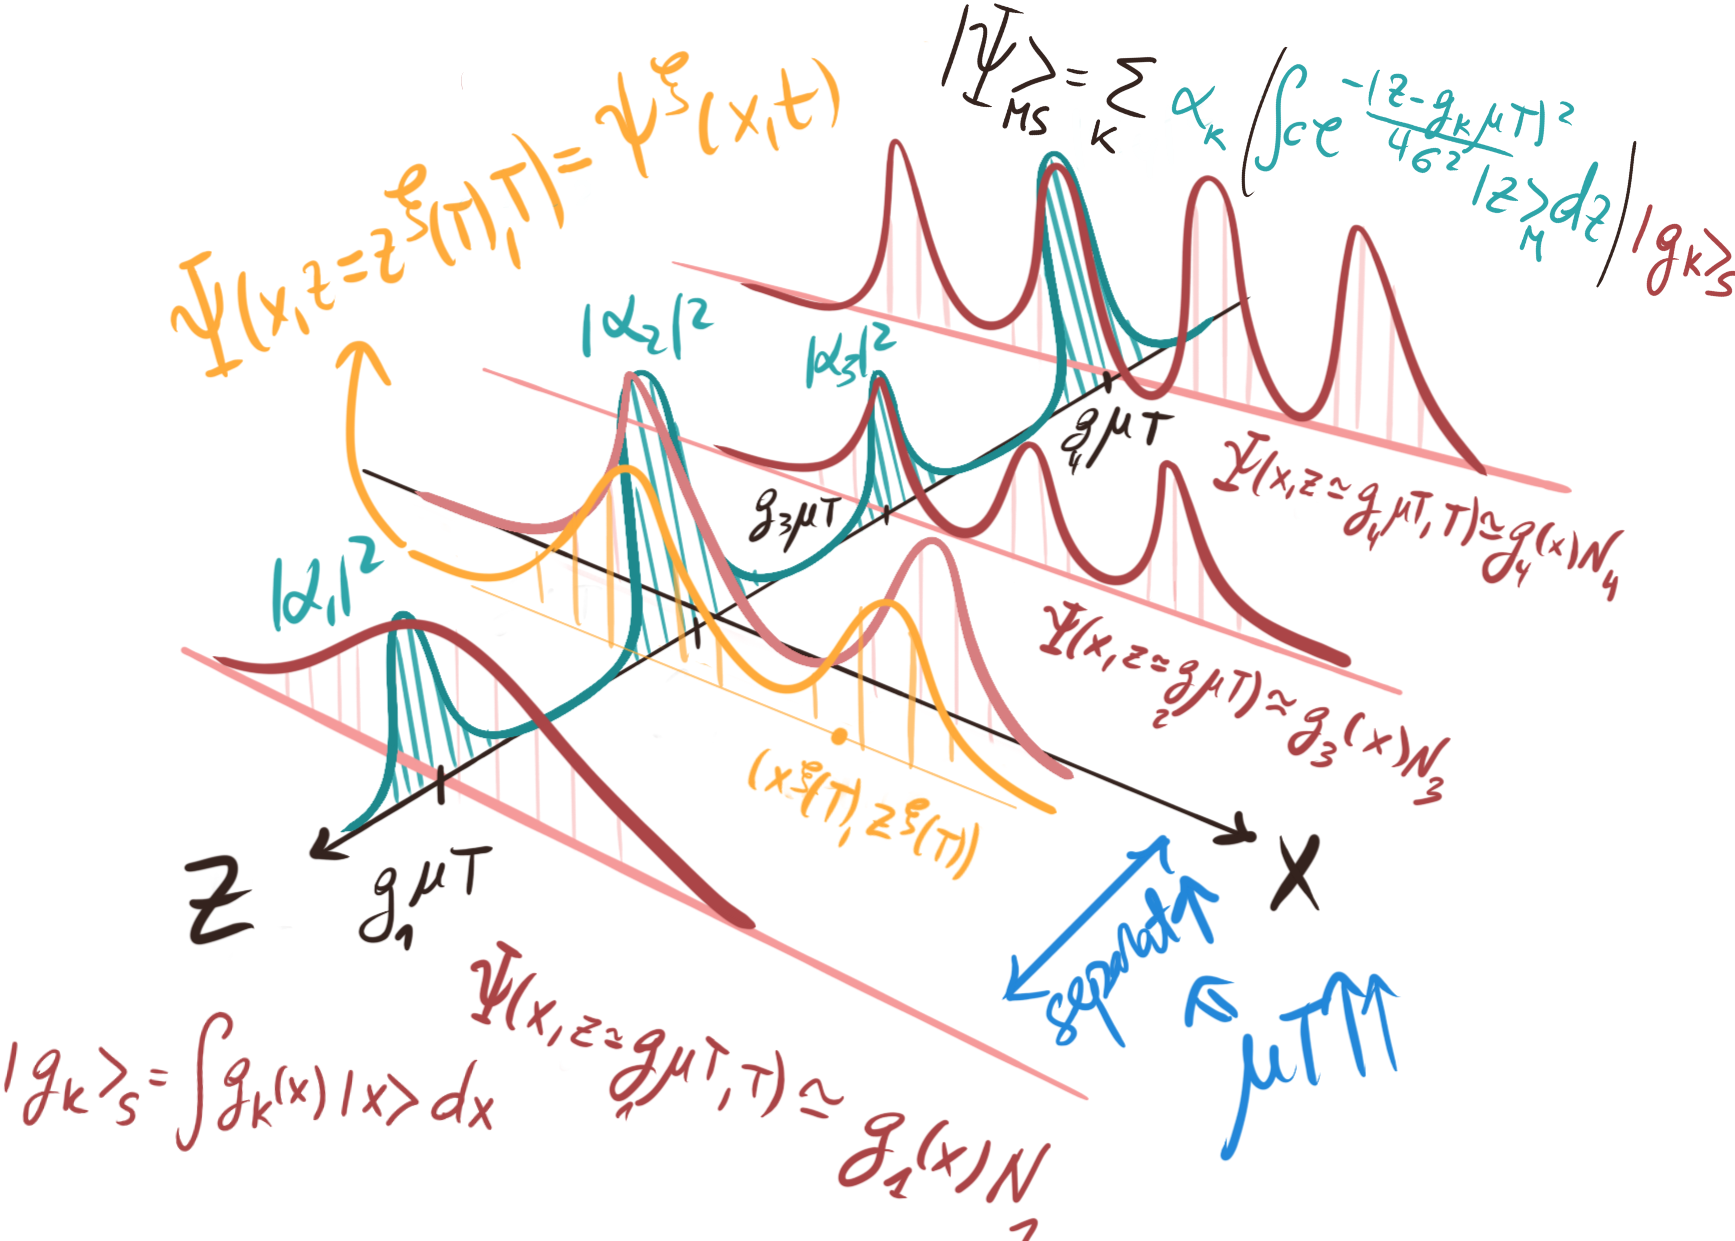
\includegraphics[width=\linewidth]{Figures/Countable.png}
%    \caption{Countable Spectrum}
%     \end{subfigure}
%\begin{subfigure}[b]{0.46\linewidth}
%    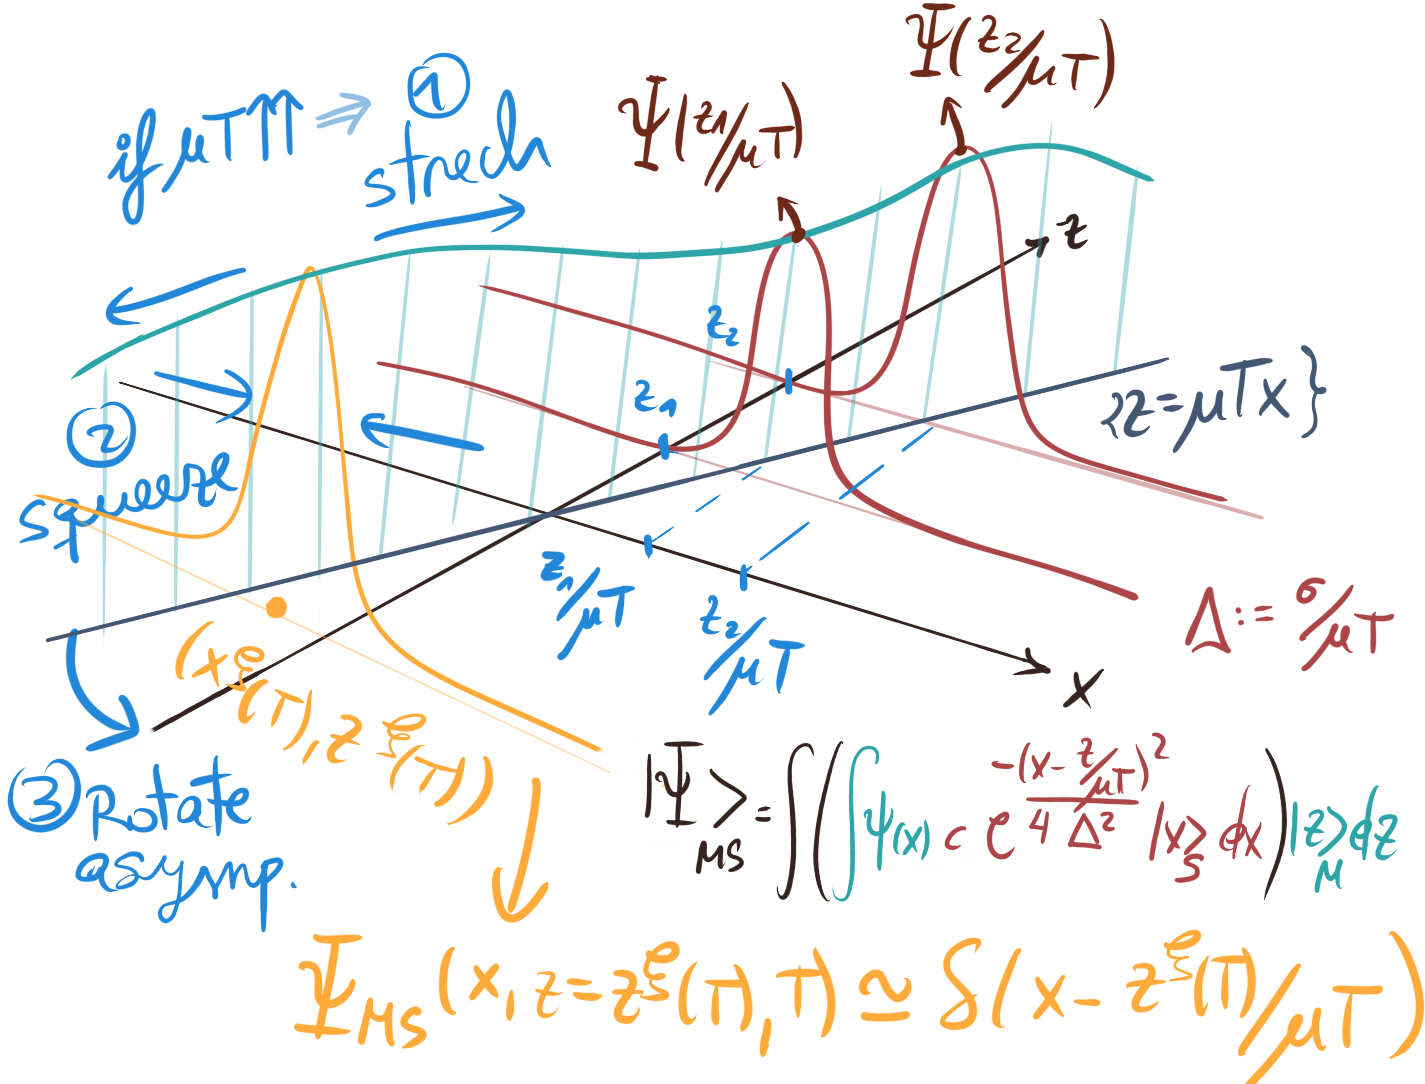
\includegraphics[width=\linewidth]{Figures/Uncountable.png}
%    \caption{Uncountable Spectrum}
%     \end{subfigure}
%   \caption{Representation of the effective collapse of a 1D ($n=1$) system, as explained in the text. In yellow the CWF of the system, which will be the EWF when normalized. $N_k$ represents the norm of the CWF. In (a), a general countable spectrum observable $\hat{B}$ is measured, in (b) a particular uncountable spectrum, the position operator $\hat{x}$, is measured. }
%  \label{fig:collapse}
%\end{figure}

% Delta sigma zati mu T jarri
% Gausianien normalizaziño konstantie
% Ezta beta karratu en el Psi!!!
% Txikixauek ekuaziñoak eta alboz jarri putse?
% Komprobeu benetan hau emon biher dabiela eta konstante de normalizaziñoa
% Ikusi lo de la norma de la  CWF!
% Putse leyendan jarri zer dan g(x). Ta jarri ke en el uncountable spectrum dibujas la variable positición, pero ke si se representa otra, g orduen tal!


In both cases, as seen from the subsytem alone, it will have looked like the unitarily evolved state $\ket{\psi}_S$ "collapsed" into one of the eigenstates of $\hat{B}_S$, with a probability equal to the pre-measurement state's projection magnitude squared $|\beta_k(0)|^2$ (or pdf $|\psi(b,0)|^2$). This EWF will now continue to be unitarily and independently evolvable (for it will be an EWF with no interaction with M). The randomness of the measurement thus, arises due to the fact that we cannot know $z^{\:(\xi)}(0)$ with an arbitrary precision, unless we made a projective measurement on it before the experiment. But such a measurement as seen, would require the coupling with another ancilla indicator, which would need to be coupled to a third ancilla, and so on until the optic nerve of the observer. This is known as the von Neumann chain of observation \cite{vonNeumann}.\footnote{In reality, we cannot really couple the apparatus dial M directly to S, nor we as observers with organic detectors are directly coupled to the dial M. Yet, we can couple S to an order of magnitude bigger ancilla $A_1$ (with say, a von Neumann Hamiltonian), which will be coupled in the same manner to a bigger ancilla $A_2$, and so on until $M$, and then until our perceptual observation, which due to the determinate Bohmian trajectory of its constituents, lets us know the result of the measurement. This discussion is in fact a restatement of the absolute uncertainty \cite{Absolute}.} The point is that a proper description of this chain, should allow us to decide where arbitrarily between the observer and S we place the effective "collapse" (as allowed by the Bohmian description), which is an ignored condition written by von Neumann himself \cite{NeumannNoCollapse} in his book on quantum mechanics.\footnote{He did not believe in a physical collapse \cite{NeumannNoCollapse}, instead he believed an explanation of the measurement should be possible setting an apparent collapse at an arbitrary point of the measurement von Neumann chain, which is what we allow with the Bohmian description. Interestingly, Bohr himself did not either believe in a physical collapse and instead owned it to the contextuality of experimental protocols \cite{Dirac}. Moreover, he believed quantum measurements should necessarily be expressed in terms of arrangements of macroscopic objects \cite{Bohr}. Funnily, both beliefs are naturally satisfied by the Bohmian description, while the orthodox collapse postulate does not imply them directly.
}\vspace{-0.1cm}

Now, either the assumption that for time $t>T$, M does not interact anymore with S, or that the environment entanglement with S is lost by some sort of thermalisation, mean that the information of the subsystem that was "leaked" to the environment M: the "empty waves", which are the rest of CWF-s that are not sliced at $z=z^{\:(\xi)}(T)$, do not interact back with the EWF of S. Any of these two assumptions thus imply that the environment effectively forgets the entanglement achieved with S. This is an environment behavior we could call memory-less or Markovian.\footnote{The evolution of macroscopically disjoint CWF-s in configuration space rapidly makes them even more disjoint \cite{Absolute}. Thus, such an assumption is reasonable in many scenarios even if the same measuring apparatus is repeatedly used.}\vspace{-0.1cm}
%\footnote{ They technically could if say, their macroscopic separation was made microscopic again. }

As a consequence, since the description of the environment M will only be useful for the measurement time interval $(0,T)$, and we can then discard it (it is Markovian for an ideal measurement), we can instead explain the apparent projection of the state of the subsystem to a subspace of its Hilbert space, with a set of effective-"collapse" orthogonal projectors $\{\hat{\Pi}_k\}_k$ without the need to explicitly formalize M \cite{Durr}. We shall not forget however that this is just a short-cut in the modeling.\vspace{-0.2cm}

\subsubsection*{1.3. The density matrix for a Bohmian}\vspace{-0.15cm}
Let us now motivate the density matrix from a Bohmian perspective. Consider the state $\ket{\psi(0)}$ and the measurement projectors $\{\hat{\Pi}_k\}_k$ for a measurement taking a time $T$, that leave $\ket{\psi(0)}$ in the possible EWF-s $\ket{\phi_k(T)}:=\hat{\Pi}_k\ket{\psi(0)}/\sqrt{P_k}$, with associated probabilities $P_k:=\bra{\psi(0)}\Pi_k\ket{\psi(0)}$. If we were not interested in a particular outcome, but we wanted to keep track of all possible post-measurement EWF-s from time $T$ to $t>T$, we could first organize them in a set of vector-probability pairs $\Lambda_{T}:=\{\big(\ket{\phi_k(T)},\ P_k\big)\}_k$, and unitarily evolve its wave-vectors independently of each other with say, $\hat{U}_{T}^{t}$, such that $\Lambda_{t}:=\big\{\big(\hat{U}^t_T\ket{\phi_k(T)},\ P_k\big)\}_k=\{\big(\ket{\phi_k(t)},\ P_k\big)\}_k$. Now, if a second measurement happened, taking time $T'$, with effective projectors $\{\hat{\Pi}'_j\}_j$, we would need to branch each of the independent states in $\Lambda_t$ into the corresponding projected states and update their probabilities: $\Lambda_{t+T'}:=\big\{ \big(\hat{\Pi}_j'\ket{\phi_k(t)}/\sqrt{P_{(j|k)}},\ P_kP_{(j|k)}\big)\big\}_{k,j}$ with $P_{(j|k)}:=\bra{\phi_k(t)}\hat{\Pi}'_j\ket{\phi_k(t)}$ the probability to get the $j$-th outcome if we obtained the $k$-th one before. Importantly, the projector $\hat{\Pi}'_j$ will always send a state to the same eigen-space, which if considered to be non-degenerate (without loss of generality), will imply we can write $\hat{\Pi}'_j=\ket{\varphi_j}\bra{\varphi_j}$. In consequence, the normalized state $\hat{\Pi}'_j \ket{\phi_k}/\sqrt{P_{(j|k)}}$ will be the same state $\ket{\varphi_j}$ for all $k$. Therefore, we could rewrite the set $\Lambda_{t+T}$ as $\Lambda_{t+T'}=\{(\ket{\varphi_j},\ P_{(j|\cdot)})\}_j$, where we gathered all the probabilities for the system to be in the state $\ket{\varphi_j}$ as $P_{(j|\cdot)}:=\sum_k P_kP_{(j|k)}$.

To have a full system description, we should also keep track of the Bohmian trajectory of the subsystem for each wave-vector. It turns out however, if we could afford the loss of ontological detail (as do the orthodox) and just cared for phenomenological probabilistic predictions like $P_k$ or $P_{(j|\cdot)}$, there is a convenient structure that works exactly as our sets $\Lambda_t$. A "matrix" operating on wave-vectors would do the same job, if we set the possible EWF-s as its composing ket-bra-s, with the probability of each EWF as coefficient. Such a "posible state-probability" pair container is what a "density matrix" \cite{vonNeumann, Durr, Holland} is all about. 
%For example, the post-measurement unconditional ensemble of state-vectors for the previous section could be written as:
%\begin{equation}\label{dens}
%\hat{\rho}_S(T) =\sum_k |\beta_k(0)|^2\ket{b_k}_S\bra{b_k}_S \quad \text{or} \quad \hat{\rho}_S(T)=\int |\psi(b,0)|^2\ket{b}_S\bra{b}_S db\vspace{-0.2cm}
%\end{equation}
If we take such a matrix for the initial state $\hat{\rho}(0):=\ket{\psi(0)}\bra{\psi(0)}$, we can get the unconditional post-measurement "container" for the first measurement as $\hat{\rho}(T)=\sum_k P_k\ket{\phi_k(T)}\bra{\phi_k(T)}$, by just applying the projectors at each side and adding the results $\sum_k\hat{\Pi}_k \hat{\rho}(0) \hat{\Pi}_k=\hat{\rho}(T)$. Then, if we apply a unitary evolution $\hat{U_T^t}$ (or in fact any linear operator) at each side of the matrix (the Hermitian conjugate in the left), we will be applying the operator to each state-vector inside it, "independently of the rest": $\hat{\rho}(t)=\hat{U}_T^{t\,\dagger}\hat{\rho}(T)\hat{U}_T^{t}=\sum_k P_k\ket{\phi_k(t)}\bra{\phi_k(t)}$. Just as we wanted. Then, for the second measurement we repeat the trick $\hat{\rho}(t+T')=\sum_j\hat{\Pi}'_j \hat{\rho}(t) \hat{\Pi}'_j=\sum_j (\sum_k P_kP_{(j|k)})\ket{\varphi_k}\bra{\varphi_k}=\sum_j P_{(j|\cdot)}\ket{\varphi_k}\bra{\varphi_k}$. Not only the time evolution and effective-collapse are easily managed with such an structure, but we can get single time measurement probabilities for an arbitrary projector $\hat{\Pi}_\alpha$ by just applying it to the matrix and computing the trace: $P(\alpha)=tr[\hat{\Pi}\hat{\rho}]$.

Although very useful for ensemble single-time statistical predictions in effective collapse scenarios, from a Bohmian point of view the density matrix has no additional relevance. Importantly, a Bohmian should always keep in mind that the microscopic detail of what is happening is lost when using only density matrices, both regarding the Bohmian trajectory and the state-vectors themselves (since different vector-probability sets yield the same matrix). Note that despite the practicity of density matrices, the state-vector and the trajectory are still the essential system state descriptors, because the Universe as a whole should be described by a certain state-vector, implying a density matrix can always be seen to represent human uncertainty about a subsystem \cite{Generalized}.\vspace{-0.2cm}


\subsubsection*{1.4. Generalized Measurements and Quantum Operations}\vspace{-0.1cm}
At this point, notice that the effective-"collapse" due to a significant separation in configuration space for different CWF groupings, is not required to be part of a measurement by an observer. It could also happen as the effect of a more general environment coupling. 
%From the perspective of the S, such an interaction with the environment could be seen as a non-unitary evolution that makes the density matrix of the system get more mixed. Yet, a requirement for this environment, that acts as an ideal projective measurement, is that the portion of the enviornment that got entangled with the subsystem and caused its effective collapse rapidly thermalizes or never again interacts with the subsystem. This is a possible narrative for a general Markovian environment.
For example, if part of the environment gets entangled with S and this environment portion is projectively measured, S will also seem to suffer an effective-"collapse", but now into non-necessarily orthogonal nor linearly-independent states (nor a number of states limited by the dimensionality of the Hilbert space of S). 

This example is in fact what is called a {\bf generalized measurement} \cite{Generalized, Durr}. Given a decomposition of an initial state $\ket{\psi}_S$ in a sum of not necessarily linearly-independent states of S and a fiducial state $\ket{\theta}_A$ for an ancilla A, by using a suitable unitary $\hat{U}_{AS}$, we could couple each state of the decomposition of $\ket{\psi}_S$ with a different state of an orthonormal basis $\{\ket{m}_A\}_m$ of A: $\hat{U}_{AS}\ket{\theta}_A\otimes\ket{\psi}_S=\sum_m \ket{m}_A\otimes \ket{\psi_m}_S$ where $\ket{\psi_m}_S:=\bra{m}_A\otimes\hat{I}_S \big(\hat{U}_{AS}\ket{\theta}_A\otimes\ket{\psi}_S\big)$ is an unnormalized S state called the $m$-th {\bf conditional state} of S ($\hat{I}_S$ is the identity). If we now perform an ideal projective measurement on A for the $\{\ket{m}_A\}_A$ basis (coupling a dial M to A and branching A in EWF-s consisting of the measured eigenstates), ancilla-subsystem (unnormalized) EFW-s $\ket{m}_A\otimes \ket{\psi_m}_S$ would be generated as a function of the Bohmian position of the dial. By the quantum equilibrium hypothesis \cite{Absolute}, the $m$-th result would be observed with a probability equal to the norm squared of its conditional state $\eta_m^2:=|\bra{\psi_m}_S\ket{\psi_m}_S|^2$. If we then set-off the interaction between A and S for all future times, the subsystem S will have seemed to "collapse" into the EWF $\ket{\psi_m}_S/\eta_m$ with probability $\eta_m^2$, since it will now evolve independently of $A$ (we assume again $A$ is an environment for the subsystem S with a Markovian behavior).

Consequently, as with the projective measurement of S, we can shortcut the formalization of A and its measurement, by just considering a set of general measurement (linear) operators on S (called POVM-s) $\big\{\hat{\Omega}_m:=\bra{m}\otimes\hat{I}_S\:\hat{U}_{AS}\ket{\theta}_A\otimes\big\}_m$, sending S states to post-measurement (unnormalized) EWF-s as: $\hat{\Omega}_m\ket{\psi}_S$. The only requirement for them is: $\sum_m \hat{\Omega}_m^\dagger\hat{\Omega}_m=\hat{I}_S$, so that the $m$-probabilities add-up to one. This is satisfied because $\hat{\Omega}_m\ket{\psi}_S=\ket{\psi_m}_S$ is the (unnormalized) post-measurement EWF of S, the squared norm of which is the probability $\eta_m^2$ to observe $m$ and thus get the EWF $\ket{\psi_m}_S/\eta_m$ for S \cite{Generalized, Durr}. The reason why such an A and $\hat{U}_{AS}$  exist for any set of linear operators $\{\hat{\Omega}_m\}_m$ satisfying the stated restriction, will be seen in a moment. Note that we could describe the post-measurement system S unconditionally, using the density matrix idea just the same way as with projective measurements, defining $\hat{\rho}_S=\sum_m \ket{\psi_m}_S\bra{\psi_m}_S$. This means we can compute it for a pre-measurement matrix $\hat{\rho}_0$ as $\sum_m \hat{\Omega}_m^\dagger \hat{\rho}_0 \hat{\Omega}_m$, where result $m$ happens with a probability $tr[\hat{\Omega}_m \hat{\rho}_0]$.

The so called partial trace operation is tigthly related to this. If the density matrix of an ancilla-subsystem composite is $\hat{\rho}_{AS}$, given an arbitrary orthonormal base of A, $\{\ket{m}_A\}_m$, the partial trace of $\hat{\rho}_{AS}$ over A is defined as: $tr_{A}[\hat{\rho}_{AS}] := \sum_k \bra{m}\otimes \hat{I}_S(\hat{\rho}_{AS})\ket{m}\otimes \hat{I}_S$ (or an integral if the "base" is made of uncountable improper states) \cite{Generalized, Durr}. We call the result, the {\bf reduced density matrix} of S. It can be easily proven that the partial trace yields the same result irrespective of the employed basis of A.\vspace{-0.1cm}

Its relation with measurements is the following one. The partial trace of M on the composite pure state $\hat{\rho}_{MS}(T)=\ket{\Psi(T)}_{MS}\bra{\Psi(T)}_{MS}$ describing the joint post-measurement state of eq.\eqref{postM1}, under the effective "collapse" conditions for $\mu,T,\sigma$, precisely yields for the subsystem S, the unconditional post-measaurement density matrix made by the possible "collapsed" EWF-s $\rho(T)_S=\sum_k |\beta_k|^2\ket{b_k}_S\bra{b_k}_S$. The same happens in any generalized measurement: the partial trace of A in the state $\hat{U}_{AS}\ket{\theta}_A\otimes\ket{\psi}_S$ following the notation of two paragraphs ago, will yield the unconditional post-measurement density matrix $\hat{\rho}_S=\sum_m \ket{\psi_m}_S\bra{\psi_m}_S$. In general, this indicates that the partial trace of an ancilla partition A of a composite ancilla A-subsystem S Hilbert space, can always be interpreted as how S would be left if an unconditional ideal projective measurement was performed on A \cite{Generalized}. Note very importantly that if the traced out partition is not projectively measured (coupling a measurement ancilla to it and evolving until macroscopic distinguish-ability is achieved) and the interaction between A and S is not "thermalised" or does not cease indeterminately, then the reduced density matrix of S will just be a "fiction". S will not evolve independently of A, as does happen in the case of a real measurement. Each CWF of S for different A states (which we placed in different slots of the matrix after partial tracing) will still interact with each other since they are not EWF-s. Yet, it is still true that for statistical measurement predictions about S, the information in the reduced density matrix will be enough. Thus, under Bohmian mechanics, the reduced density matrix is in general just a "ficticious" "how the subsystem S would be left if", useful to predict single-time measurement statistics on S. %In general though, it will be "ficticious" representation of how S would be left if the rest was unconditionally projectively measured. %Unless of course, a real unconditional measurement of A is performed (by an outer environment or by an observer) and the A-S interaction ceases. Interesting enough, the observable measured on the traced out partition is irrelevant for the resulting reduced density matrix, which is what allows the versatility of the so called pure unravellings.


In order to finish integrating the density matrix formalism and any general quantum operation (including the generalized measurements) with this Bohmian view, we can invoke the Gelfand-Naimark-Segal theorem \cite{GNSTheorem, Generalized}. By this theorem, we can assure that for any most general operation we can perform on a density matrix $\hat{\rho}_S$ of a system S (any complete-positive, convex linear and not trace increasing superoperator acting on S), say, for the operation $\mathfrak{S}$, there exists at least an ancilla system A with a pure state $\ket{\theta}_A$ and a coupling unitary evolution $\hat{U}_{AS}$ such that:\vspace{-0.15cm}
\begin{equation}
\mathfrak{S}[\hat{\rho}_S]=tr_A\qty[ (\hat{\Pi}_A\otimes \hat{Id}_S)  \hat{U}_{AS}\qty(\ket{\theta}_A\bra{\theta}_A\otimes \hat{\rho}_S)\hat{U}_{AS}^\dagger]
\end{equation}
which can be interpreted as a unitary coupling of the initially independent S and A, and posterior partially unconditional ideal projective measurement of $A$ (where only the eigenstates of non-null eigenvalue of $\hat{\Pi}_A$ are left and the rest are discarded). We have given a Bohmian view for all of them, so this closes the whole (non-relativistic) picture. In particular, if the coupling of S and A perfectly entangles the eigenstates of $\hat{\Pi}_A$ with an orthonormal basis of S, this will be a projective measurement of S. In the trivial case where $\hat{U}_{AS}=\hat{U}_A\otimes\hat{U}_S$ and $\hat{\Pi}_A=\ket{\theta}_A$, it will just be the Schrödinger unitary evolution of S. Else, it will be a generalized measurement of S.  Interestingly, this is a practical method used by quantum engineers to physically implement arbitrary quantum operations $\mathfrak{S}$ in a lab.


\subsection*{2. Practical Bohmian Mechanics: Markovianity and SSE-s}
Following the Markovianity idea we pragmatically defined earlier, we could call a Markovian open quantum system, any evolution of the reduced density of a subsystem S that could be equivalently interpreted as if a different portion of the environment (a different ancilla) instantly got coupled every $\Delta t$ with S and was then ideally measured, in a way that this ancilla never again interacted with the system (or their entanglement was somehow "thermalised" before their next interaction) \cite{QuantumTrajs}. This is equivalent to a generalized measurement of S every $\Delta t$. Among others, the "Past-Future Independence" definition of Markovianity by Ref. \cite{MarkovianityDefs}, perfectly matches this view.

In fact, as shown by Ref. \cite{continousMeas}, such a continuous monitorization of different ancillas that get coupled to the subsystem at each time, can be used to derive dynamical equations for the reduced density matrix of a subsytem in a Markovian environment, a type of so called Lindblad master equations \cite{Generalized, MarkovianityDefs}. Then the generalized derivation of an arbitrary Markovian environment Lindblad master equation, requires the consideration of several simultaneous continuous measurements for different properties of the bath \cite{continousMeas, MarkovianityDefs}. The same idea for Markovianity still holds.

The fact that the dynamics of the reduced density matrix of a subsystem can be understood in these terms means that instead of trying to solve the Markovian master equation, we could do the following. Find an observable $W$ for some (fictitious or not) environment ancillas, E, ancillas that get entangled with S and are then projectively measured, producing the same average (unconditional) effect on the reduced density of S as the predicted one by the master equation (which is always possible for a Markovian E as said). Then, we could evolve a pure state-vector of S choosing at each projective measurement of the bath, one of the possible stochastic conditional states. This would generate a linked in time subsystem pure state $\ket{\psi_{w(t)}(t)}_S$, associated to the result of a certain continuous measurement (or unravelling) of the bath ancillas: $w(t)$\footnote{At each time a different generalized measurement is performed on S, meaning the stochastic trajectory $w(t)$ reflects the Bohmian positions of different measurement dials at each $\Delta t$. Its non-differentiability is thus unproblematic.}. This pure state is called a {\bf quantum trajectory}, linked to a "noise realization" $w(t)$ for its environment \cite{Generalized, MarkovianityDefs, QuantumTrajs}. As we saw previously that the reduced density matrix of a subsystem is how it would be left if an unconditional ideal measurement was performed on the rest of the system, this tells us that we should be able to recover the reduced density for S by averaging the ensemble of all possible quantum trajectories for the unraveling of the $W$ observable of the bath ancillas \cite{MarkovianityDefs,QuantumTrajs}:\vspace{-0.17cm}
\begin{equation}
\hat{\rho}_S(t):=tr_{ES}[\hat{\rho}_{ES}(t)]=\mathbb{E}_{w(t)}\qty[\ket{\psi_{w(t)}(t)}_S\bra{\psi_{w(t)}(t)}_S] \vspace{-0.13cm}
\end{equation}
Computationally, this means that if we got an equation ruling the stochastic time evolution of a pure quantum trajectory $\ket{\psi_{w(t)}}_S$ and its noise realization $w(t)$, we would be able to compute in parallel the density matrix using simpler data structures (vectors) \cite{MarkovianityDefs, QuantumTrajs}. Additionally, the obtained reduced density matrix is necessarily positive definite by construction. Equations of these kind are the so called, {\bf Stochastic Schrödinger Equations} (SSE-s) \cite{Generalized, continousMeas}. Note that such a pure state trajectory for a Markovian environment E, can always be physically interpreted in the orthodox explanation, as a so called pure unravelling \cite{MarkovianityDefs} (where one would invoke the collapse at each $\Delta t$). In the Bohmian view a quantum trajectory is exactly a normalized CWF of the subsystem S (in ket notation), which every significant $\Delta t$ is converted into an EWF (thus the normalization).\vspace{-0.05cm}

%From our Bohmian perspective, this works because at each time $t$, the ideal measurement of the environment portion A entangled with the system S, makes the A-S CWF obtained by conditioning the A-S-measurement-apparatus wavefunction to the dial position $w(t)$ be converted into an EWF, just as explained when describing the narrative for POVMs. As was clear for POVMs in general, notice again that the measured property of the bath, indicated by $w(t)$, does not need to be its position (even in Bohmian mechanics). It is the position of the dial measuring the property of the bath, that must be a position (which is actually what $w(t)$ is in each time, assuming the Bohmian postulate that a measurement is always a position measurement in the end). 

However, what if we had an environment E that gets entangled with S, but which never really allows us to consider an effective collapse? What if the different CWF-s of the subsystem S, were allowed to interact in any future time, and were not converted into EFW-s every $\Delta t$? That is, what if the "quantum trajectories" could interact between them, such that the evolution of each of them depended on the rest? Then "the information leaked" onto the environment from S (the "empty waves"), would be able to affect back S in any significant future time for S. Such an environment with "memory" of the entanglement achieved with S could be called a non-Markovian environment \cite{MarkovianityDefs}. Then, it turns out that from a Bohmian interpretation, we could still continue talking about "pure state quantum trajectories", which would be the CWF-s for the subsytem S (in any desired representation), conditioned on a position for the environment interacting with S (or conditioned on the positions of dials coupled with arbitrary observables of the environment ancillas interacting with S) \cite{NMisModal, interpretSSE}. Since measurement and collapse are just described as another unitary evolution of the whole, and the positions are ontologically real at all times, then there is no interpretative issue.\vspace{-0.05cm}

Contrarily, in the orthodox view, a CWF (normalized or not and in any representation basis), does not have a physical interpretation, unless it is an EWF, say, unless the conditioning variable is projectively measured. As a consequence, if a SSE is found for a non-Markovian dynamical equation ruling a reduced density matrix, the conditional pure state evolved by the SSE, in the orthodox view, can only be understood as the state in which S would be left on, if the environment E was measured...but since it is non-Markovian, we cannot assume E is being projectively measured! If it was, the evolution of the state would be pretty different (we would neglect part of the quantum wholeness, the interaction between the CWF-s stacked along the coordinates of E). Thus, the linking of such states in time, can only be understood if we get out of the orthodox and use concepts like the CWF of the Bohmian view \cite{NMisModal, interpretSSE}. Of course, mathematically, one could derive such non-Markovian SSE-s as pragmatical computational tools to reconstruct the reduced density matrix, but one would need to avoid any additional consideration for the quantum trajectory (like two-time correlation computations), unless one accepts some sort of ontological reality (independent of measurement) for the conditioning property of the environment.

From the Bohmian perspective it is easy to notice why SSE-s for non-Markovian environments will not be exact in general. One of the main properties a SSE needs to have is that it should allow the time evolution of a single conditional state independently of the rest of possible conditional states. This is precisely to ask that there is no quantum influence between adjacent CWF-s, influence which as explained in the beginning, is the main signature of quantum mechanics (the quantum wholeness). In fact, this is asking for these CWF-s to be EWF-s as we saw, which would then allow a Markovian interpretation for the SSE, and thus would imply a contradiction. Yet, SSE-s that {\bf approximate} the dynamics for ad-hoc cases are indeed possible in non-Markovian environments \cite{ Diosi, WisemanSSE, Thz}. This is because an ensemble of CWF-s does not need to be an ensemble of EWF-s to allow the computation of the reduced density matrix at each time!\footnote{In fact, a whole set of CWF-s, if the system state was not mixed, would also allow the reconstruction of the full environment-system wavefunction! In which case a reduced system density matrix would not even be necessary.} 

To see that this is so, independently of the nature of the environment, let us prove it for an arbitrary composed pure state (the generalization to mixed states is then trivial). Given the arbitrary state $\ket{\Psi}_{ES}$ for the environment E and system S, with position observables $\vec{y}$ and $\vec{x}$ respectively, just as introduced in the beginning\footnote{Note that since Bohmian trajectories do not cross each other in configuration space, if we sampled only Bohmian trajectories for which $\vec{x}(0)$ is a single position $\vec{a}$, at each time, we would still have a CWF per each position in $\vec{y}$. Thus, we have that the states $\qty{\ket{\psi^{y(\xi,t)}(t)}_S:=\bra{y(\xi,t)}_A\ket{\Psi(t)}_{AS};\ \vec{x}(0)=\vec{a}}_{y\in\R^{N-n}}$ are all the possible slices of the $\vec{y}$ axis.}:\vspace{-0.2cm}
\begin{equation}
\ket{\Psi(t)}_{AS}=\int\ket{\vec{y}^{\:\xi}(t)}_A\otimes \ket{\psi^\xi(t)}_S d\xi = \int\ket{\vec{y}}_A\otimes \ket{\psi^{y(\xi,t)}(t)}_S dy
\end{equation}
Then tracing out A in $\hat{\rho}_{AS}(t)=\ket{\Psi(t)}_{AS}\bra{\Psi(t)}_{AS}$, would yield the reduced density for S:
\begin{equation}\hspace{-0.2cm}
tr_E\qty[\hat{\rho}_{AS}(t)] = \int\bra{\vec{y}}\hat{\rho}_{AS}(t)\ket{\vec{y}}dy = \int \ket{\psi^{y(\xi,t)}(t)}\bra{\psi^{y(\xi,t)}(t)} dy = \mathbb{E}_{y(\xi,t)}\qty[\ket{\psi^{y(\xi,t)}(t)}\bra{\psi^{y(\xi,t)}(t)}]
\end{equation}
Which proves the ensemble average of the CWF-s reproduces the reduced density at any time.\vspace{-0.15cm}

This clear narrative in terms of Bohmian CWF-s for non-Markovian open quantum systems is not only theoretically insightful, but is a {\bf practical} tool to look for reasonable SSE-s. To exemplify this, let us describe a practical use-case we developed.\vspace{-0.2cm}

\subsubsection*{2.1. Non-Markovian SSE for nano-electronic devices operating at THz frequencies}\vspace{-0.15cm}
%In the pragmatical view we have mentioned about Markovian open quantum systems, we said the dynamics should be interpretable as if every $\Delta t$ a POVM (instantaneously for S) took place. This means that in such a picture, the entanglement and interaction bewteen the subsystem and the enviornment should decay in a time scale $\tau_{decay}$ much smaller than any characteristic time scale for the subsystem $\tau_S$ (related with $\Delta t$), $\tau_S>>\tau_{decay}$. However, 
In the first section, we arrived at an exact system of equations following equation \eqref{SE.GJ}, that described the general time evolution of CWF-s in arbitrary settings. In principle, in those equations the CWF of the subsystem S and its environment E are coupled at all times, not only between them, but also with the rest of possible CWF-s (signature of the non-Markovianity). However, for specific scenarios, we can make educated guesses for the quantum correlation terms $G$ and $J$ \eqref{G.Bohm},\eqref{J.Bohm}, and the classical potential $U$, to render a SSE for individual CWF-s of the subsystem S. Thus, this is a general framework to look for SSE-s. Let us describe now an example use-case.

For nano-scale electronic devices operating at very high frequencies (in the order of THz), both the relevant dynamics of the active region electrons and the current measurement coupling times are below picoseconds, implying Markovian assumptions for the coupling are meaningless \cite{Thz}. This problem for a two-terminal nano-electron device is approximated in the BITLLES simulator \cite{tdp,Pois,Thz}, as an application of the mentioned method. For this, the classical potential is evaluated as a solution of the Poisson equation \cite{Pois}, while $G$ and $J$ are modeled by a proper injection model \cite{inject} as well as proper boundary conditions \cite{boundary1, boundary2} that include the correlations between the active region of the two-terminal nano-device and the reservoirs. Even electron-phonon decoherence effects can be included \cite{eph}.

The electrons contributing to the electrical current, the observable of interest, are mainly the $n/3$ electrons in the active region of such a nano-device, thus we consider the active region is the subsystem S of interest. The number $n/3$ fluctuates in time as there are electrons entering and leaving this region. Such a "creation and destruction" of electrons, from the point of view of S, leads to an abrupt change in the degrees of freedom of its CWF. This problem can be circumvented in Bohmian mechanics by decomposing the CWF of S, $\psi^{\xi}(\vec{x},t)$, into a set of CWF-s for each electron. That is, for each of the $n/3$ electrons of positions $\vec{x}_k:=(x_{3k+1}, x_{3k+2}, x_{3k+3})$ with $k\in\{0,..,n/3-1\}$, we define a single-particle CWF $\phi_k^\xi(\vec{x}_k, t):=\psi^{\xi}(\vec{x}_k, \vec{x}_{\neg k}=\vec{x}_{\neg k}^{\:\xi}(t),t)$ with $\vec{x}_{\neg k}=(\vec{x}_1,..,\vec{x}_{k-1}, \vec{x}_{k+1}, ...,\vec{x}_{n/3})$. Then, we can consider a set of $n(t)/3$ equations like \eqref{SE.GJ}, one for each of the electrons, to evolve each single-particle CWF $\phi_k^\xi$. Note that what we have just done is to consider S, the non-Markovian open quantum system, as itself composed of several open quantum systems that will interact with each other in a non-Markovian way. This turns out to simplify the problem.

Now, the active region of the electron device S, is connected by a macroscopic cable A (representing the portion of the environment that gets entangled with S) to an ammeter M (acting as a measuring apparatus). The electrical current read by the Bohmian position of the dial in the ammeter M is the phenomenological observable we want to predict. Thus, in principle the evaluation of the electrical current should require keeping track of all the environment degrees of freedom for A and M. However, it is known that the total current density, defined as the sum of the particle and displacement currents, is a divergenceless vector \cite{diver1, diver2}, which makes the total current evaluated at the ends of the active region S be equal to the total current evaluated at the cables A. It is additionaly known \cite{equiv} that since the cables, unlike the active region, have macroscopic dimensions, the current at the ends of the active region S is only due to the electrons in S (plus a nearly white noise). This is qualitatively because the electrons in the metallic cables have a very short screening time, meaning the electric field generated by an electron in the cable spatially decreases rapidly due to the presence of many other mobile charge carriers in the cable that screen it out. Thus, the contribution of these outer electrons of A to the displacement current at the border of the active region is negligible \cite{neg}. Therefore, the variable of the environment associated to the total current $z(t)\equiv I(t)$ can indeed be equivalently computed at the boundary of S. Finally, such a current (its expected value) is computable from the Bohmian trajectories of the electrons in the active region S, as we will explain in Section 3. 

In Ref. \cite{Thz} we provide some numerical results demonstrating the ability of the presented method, by simulating a two-terminal electron device whose active region is a graphene sheet, contacted to the outer by two (ohmic) contacts. See Figure \ref{fig:fig}. %Here, to further take into account the electromagnetic environment of the electron device, we model the interaction between the graphene device and the outer environment through a resistor and a capacitor in series. The details are found in the mentioned article. 
\begin{figure}[h!]
  \centering
  \hspace*{-0.5cm}
    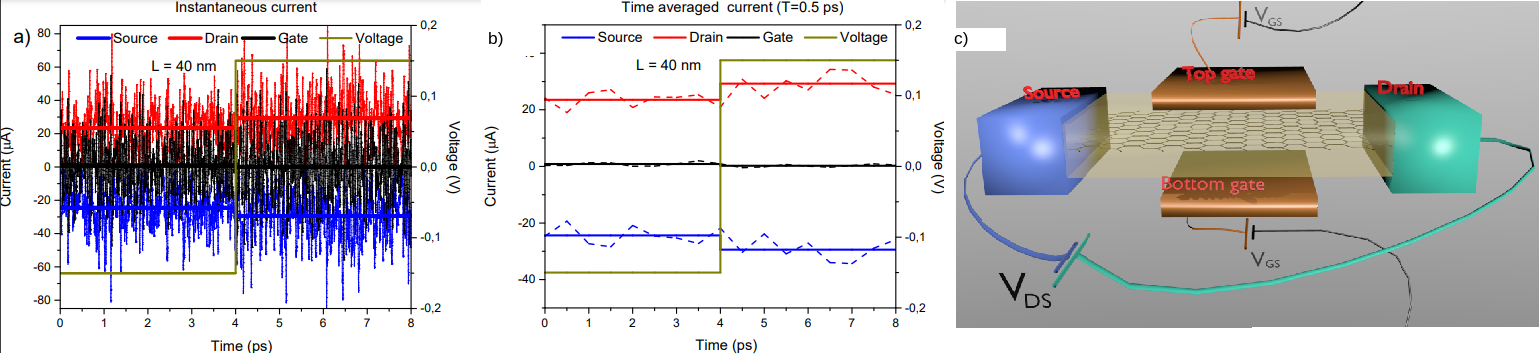
\includegraphics[width=1.05\linewidth]{Figures/abc.png}
   \caption{Tal tal tal.}
  \label{fig:fig}
\end{figure}

%\newpage
%\subsubsection*{2.2. Towards another general framework to look for position SSE-s}
%We have developed a second framework to look for SSE-s (equations to evolve CWF-s independently), based on the Born-Huang ansatz of the full wavefunction, at the cost of having a suitable guess for the conditional energy eigenstates of the relevant parts of the environment. For this, given the full, subsystem-environment Hamiltonian $\hat{H}(\vec{x},\vec{y},t)=\sum_{k=1}^N \frac{-\hbar^2}{2m_k}\pdv[2]{}{x_k} + U(\vec{x},\vec{y},t)+V(\vec{x},t)$,\footnote{The classical potentials $U,V$ are allowed to have explicit time dependences to account for classical interactions with the rest of the environment.} we can define the transversal section Hamiltonian as $\hat{H}_x(\vec{y},t):=\sum_{k=m+1}^N\frac{-\hbar^2}{2m_k}\pdv[2]{}{x_k}+U(\vec{x},\vec{y},t)$. Then, we define the set of eigenstates $\{\Phi^j_x(\vec{y},t)\}_j$ with eigenvalues $\{\varepsilon_x^j(t)\}_j$, parametrized by the chosen section $\vec{x}$, to be the solution of: $\hat{H}_x(\vec{y},t)\Phi^j_x(\vec{y},t)=\varepsilon_x^j(t)\Phi^j_x(\vec{y},t)$. We call these states $\Phi^j_x(\vec{y},t)$, the transversal section eigenstates (TSE). Since the hermiticity of the operator $\hat{H}_x(\vec{y},t)$ implies the TSE-s form an orthonormal basis for the Hilbert space of $\vec{y}$ at each $\vec{x}$, we could expand the following ansatz: $\Psi(\vec{x},\vec{y},t)=\sum_j \Lambda^j(\vec{x},t)\Phi_x^j(\vec{y},t)=\sum_j \varphi_j(\vec{x},\vec{y},t)$, with $\Lambda^j(\vec{x},t):=\int\Phi^j_x(\vec{y},t)\Psi(\vec{x},\vec{y},t)dy$ the projection coefficients and $\varphi_j(\vec{x},\vec{y},t):=\Lambda^j(\vec{x},t)\Phi^j_x(\vec{y},t)$.

%Now, using this expansion in the Schrödinger Equation, and evaluating the full wavefunction along the trajectory for the environment $\vec{y}=\vec{y}^{\:\xi}(t)$\footnote{In reality, we could choose any trajectory we like for the environment if we are not interested in computing Bohmian trajectories. Thus, it could be the result of a measurement of the environment, or just a set of trajectories that leads us to the reconstruction of the reduced density with the least number of them.}, we can get by denoting $\varphi^k_\xi(\vec{x},t):=\varphi^k(\vec{x},\vec{y}^{\:\xi}(t),t)$:
%\begin{equation}
% i\hbar\pdv{}{t}\varphi^k_\xi(\vec{x},t)=\qty[-\sum_{s=1}^m\frac{\hbar^2}{2m_s}\pdv[2]{}{x_s}+ \varepsilon^k(\vec{x},t)+V(\vec{x},t)   +i\hbar \dv{}{t}log(\Phi^k_x(\vec{y}^{\, \xi}(t),t))]\varphi^k_\xi(\vec{x},t)+
%\end{equation}
%$$
%\hspace{-0.4cm}+\sum_{j=0}^\infty\sum_{s=1}^m \frac{-\hbar}{2m_s}\qty( \frac{1}{\Phi^j_x(\vec{y}^{\, \xi}(t),t)}\pdv[2]{\Phi^j_x(\vec{y}^{\, \xi}(t),t)}{x_s}+2\pdv{}{x_s}log(\Phi^j_x(\vec{y}^{\, \xi}(t),t))\qty[\pdv{}{x_s}-\pdv{}{x_s}log(\Phi^j_x(\vec{y}^{\, \xi}(t),t))] )\varphi^j_\xi(\vec{x},t)
%$$
%Because the CWF for the subsystem can be recovered from $\psi^\xi(\vec{x},t)=\sum_j \varphi^j_\xi(\vec{x},t)$, we have obtained a set of {\bf exact} linear equations involving only $n$ dimensional states (instead of $N$) that allow the evolution of single CWF-s. In principle, since a general Hilbert space will need to have a countably infinite number of orthonormal states in a basis, it would be a set of infinite number of equations. However, we shall reasonably truncate the expansion of the CWF at a relatively low fixed point (at which for example the norm of the CWF surpasses a certain threshold), or even allow it to vary in time. If so, the difficulty of these equations would only relay on the knowledge of the TSE-s $\Phi^j_x(\vec{y},t)$. The point is that providing educated guesses for them seems to be more reasonable than guessing for $G$ and $J$ \eqref{G.Bohm}, \eqref{J.Bohm}. Thus, this might be the starting point for the derivation of SSE-s for a particular non-Markovian environment, which as said previously, will need to be approximate in general.  \vspace{-0.2cm}

 
\subsection*{3. Practical Bohmian Mechanics: Accessible "Unmeasured System" Properties}

Under the orthodox {\em eigenstate-eigenvalue link} we can only say a quantum system {\bf has} a property when its wavefunction is an eigenstate of the operator related to that property. This implies, that when a wavefunction is in general in a superposition of different eigenstates, nothing can be said about the "reality" of its related property. Since a strong measurement, as we have seen, always forces the system to adopt an eigenstate, while the unitary evolution in the meantime, will cause a superposition in general, we are only allowed to speak about properties of {\bf measured} quantum systems. However, this implies an engineer cannot talk about the properties, nor even the same "reality", of the electrons in the nanometric active region of a device, since if anything, it is the cables coupled to that active region that are measured with say, an ammeter. This leaves the electrons only weakly measured and thus in general, their wavefunction, in a superposition. This impasse implies practical difficulties, for instance when trying to measure the maximum working frequency of nano-scale transistors to test the performance of modern computers \cite{modern}. For this, the time spent by electrons in the active region of the transistors, their "dwell time", must be measured. The eigenstate-eigenvalue link would force us to place position detectors in the two ends of the active region. However, the obtained metric would be meaningless, since in operation no computer has such detectors at the ends of its transistors \cite{tunnel1, tunnel2}, and every measurement produces a backaction in the system, causing its subsequent evolution to be different than otherwise, as we have seen. Therefore, {\bf three impasses} need to be clarified here. First, is there a way in which we can meaningfully talk about "unmeasured system"\footnote{A system that is not being measured, e.g. a closed system evolving without quantum interaction with its environment.} properties, and even still be in accordance with orthodox phenomenology? Second, are these "unmeasured system" properties experimentally accessible? And third, can these properties be employed to operationally compute practical information, or are they mere philosophical reliefs?

Before proving Bohmian mechanics gives an affirmative answer to the three questions, let us further motivate such a quest for non-{\em contextual}\footnote{Contextual means it depends and implies the environment used to convey the information to the observer.} properties or equivalently, "unmeasured system" properties. It turns out the contextuality of the quantum measurement, no matter how weak it is, as we have shown, introduces an inescapable backaction in the system (effective collapse) that disrupts its future evolution. Under the eigenstate-eigenvalue link this poses a clear impasse when looking for two time information about the system evolution. This extends the dwell time problem for instance to thermodynamoics, where {\bf work} is by definition a dynamical property implying at least two times. The mentioned contextuality issue has led to a "no-go" theorem \cite{nogo} stating that there cannot exist a quantum work superoperator that simultaneously satisfies all the physical properties required from it. Other history dependent thermodynamic properties suffer from the same issue \cite{workPb1, workPb2}: a definition of them always seems to be dependent on a particular measuring scheme, which causes as many quantum work definitions as, say, acceptable measurement fiducial states exist. But more in general, {\bf two time correlations} of non-commuting observables, say $F$ and $B$, independently of a measuring device, are hard to be defined. We could correlate the result of a strong measurement of $F$ at time $t_1$ and a strong measurement of $B$ at time $t_2$, but since the measurement at $t_1$ will project the state to different EWF-s, the backaction of the measuring device will be obvious. In fact, even numerically it seems hard to be well defined. If their operators do not commute, $\langle \hat{B}(t_2)\hat{F}(t_1)\rangle$, in the Heisenberg formalism, will give a complex number in general. We could just take the real part $\mathbb{R}e \big\{\langle \hat{B}(t_2)\hat{F}(t_1)\rangle\big\}$, which turns out to be the correlation of a weak measurement \cite{Weak} of $F$ at time $t_1$ and a strong measurement of $B$ at time $t_2$. Yet, as shown in \cite{spin}, even an ideally weak measurement does in fact perturb the system in a way that is dependent, for example, on the particular fiducial state employed for it.  Then, are we fundamentally forbidden to access dynamical information about the "unmeasured" system? \vspace{-0.15cm}

%\subsubsection*{ 3.1. Measurement operators defined in terms of Bohmian trajectories}
\subsubsection*{3.1. Breaking Impasse 1: General unmeasured system properties }\vspace{-0.15cm}

Let us first clarify what is exactly the information we gain when we measure a quantum system and whether this information is about the pre-measurement/"unmeasured" system, or the post-measurement system. Consider an observable operator $\hat{B}=\sum_b b\ket{b}\bra{b}$, with $\{\ket{b}\}_b$ an orthonormal basis and $\ket{\psi}$ the wavefunction of the pre-measurement system. We have seen that measuring $B$ will lead the system to the {\bf post}-measurement state $\ket{b}$ linked with the measured $b$, which will happen with a probability $|\bra{b}\ket{\psi}|^2$ due to the {\bf pre}-measurement state. Thus, on the one hand, three things about the post-measurement system are revealed: its state $\ket{b}$, the measured value $b$, and if it was a generalized measurement, the wave-vector in which the system coupled to the measured ancilla is left by the effective collapse of the ancilla. About the pre-measurement system on the other hand, we can seemingly only know, if we repeat the experiment enough times, the probabilities of each outcome, which are the magnitudes of the pre-measurement state's projection onto the possible post-measurement states $|\bra{b}\ket{\psi}|^2$. But if a "measurement", as Bell said \cite{Bell}, has the connotation of unveiling or revealing information about the ({\bf pre-}measurement) system, becasue else, we should just call it an "experiment": are these magnitudes the only thing we can really know about the unmeasured system? The answer by a naive orthodox would be no, if we also use the value $b$ signaled by the dial. We could for example compute the expected value for the observed $b$, which will yield the same value as the expectation $\langle \hat{B} \rangle:=\bra{\psi} \hat{B} \ket{\psi}$ that can be computed non-contextually with the pre-measurement state $\ket{\psi}$. However, the eigenvalue-eigenstate link would prevent us considering $b$ as a property of the unmeasured system, and thus $\langle \hat{B} \rangle$ as well. In all case they are a property of the measured (or post-measurement) system. What about a Bohmian? For a Bohmian, if $\hat{B}$ is a function of the position operator $f(\hat{x})$, then $b$ is the post-measurement property $B$ related with the Bohmian trajectory (say, its position), and since the trajectory must be continous in time, at least it will be linked with the pre-measurement property $B$. However, if we take a general operator $\hat{B}$ that does not commute with the position (like the energy or momentum operators), we could think that the measured $b$ is just a property related with the wavefunction piloting the trajectory, not the trajectory itself. Yet, Bohmian mechanics is not limited to this. It might not be well known, but it is indeed possible to consider that any orthodox observable operator is due to a defined property of the underlying position trajectory \cite{DevInPosition1, DevInPosition2}. This will be what will break the "unspeakables". Let us review how.

%\footnote{Which, as will be explained later, is the weak value \cite{Weak} of $\hat{B}$ for the state $\ket{\psi(t)}$ at time $t$, post-selected at $\vec{x}$} 
Given any arbitrary (Hermitian) operator $\hat{B}$, describing the observable property $B$ for the subsystem S, with normalized EWF $\ket{\psi(t)}$, let us first blindly define the function $C^{\psi}(x,t):=\frac{\bra{\vec{x}}\hat{B}\ket{\psi(t)}}{\bra{\vec{x}}\ket{\psi(t)}}$. Then, we could define a real function $\B^\psi(\vec{x},t):=\mathbb{R}e\{C^{\psi}(x,t)\}$, and see what happens if we understand it as the property $B$ of the Bohmian trajectory passing from $\vec{x}$ at time $t$, be the system measured or not. It seems just a cumbersome definition, yet, write the expected value for $\hat{B}$  as a function of $C^\psi(x,t)$:
\begin{equation}
\langle \hat{B}\rangle(t)= \bra{\psi(t)}\hat{B}\ket{\psi(t)}=\int \bra{\psi(t)} \ket{\vec{x}}\bra{\vec{x}}\hat{B}\ket{\psi(t)}dx =  \int |\psi(\vec{x},t)|^2C^\psi(\vec{x},t)dx
\end{equation}
This means that the spatial average of the (possibly complex) $C^\psi(\vec{x},t)$ gives at all times, the same expected value for the observable $\hat{B}$ as the one given by the $\bra{b}\ket{\psi(t)}$ coefficients. Nice, but here comes the most interesting point: since $\hat{B}$ is an observable, its expected value will be a real number, meaning that $\langle \hat{B}\rangle=\mathbb{R}e\{\langle \hat{B}\rangle\}$, and thus, it could equivalently be computed from $\B^\psi(\vec{x},t)$:
\begin{equation}
\langle \hat{B}\rangle(t)=\int |\psi(\vec{x},t)|^2\B^\psi(\vec{x},t)dx= \lim_{|\Sigma|\rightarrow \infty}\frac{1}{|\Sigma|} \sum_{\xi\in\Sigma} \B^\psi(\vec{x}^{\:\xi}(t),t)
\end{equation}
where we additionally used the quantum equilibrium hypothesis \cite{Absolute} for the set of trajectories $\{\vec{x}^{\:\xi}(t)\}_{\xi\in\Sigma}$ sampled in independent repetitions of the experiment. This equation means that the real property $\B^\psi(\vec{x}(\vec{\xi},t),t)$ of the $\vec{\xi}$-th Bohmian trajectory, averaged over the ensemble of possible trajectories, gives the same value as the operator's expectation. Still, $\B^\psi$ seems to be just an ad-hoc definition for this to be satisfied. The true hit comes with the following: what would the suggested Bohmian property related with $B$ be if the system state, $\ket{\psi}$, was an eigenstate of $\hat{B}$ with eigenvalue $b$?
\begin{equation}
\B^\psi(\vec{x})=\mathbb{R}e\qty{ \frac{\bra{\vec{x}}\hat{B}\ket{\psi}}{\bra{\vec{x}}\ket{\psi}} } = \mathbb{R}e\qty{ \frac{\bra{\vec{x}}\ket{\psi}b}{\bra{\vec{x}}\ket{\psi}} }=b
\end{equation}
This suggests $\ket{\psi}$ is an eigenstate of $\hat{B}$ if and only if it is a state for which every Bohmian trajectory has the same value of the property $\B^\psi$. On the one hand, this tells us that philosophically, the $b$ indicated by the dial of a projective measurement, can always be considered to be a property of the Bohmian trajectory, even when its operator does not commute with position. On the other hand, operationally, it is a tool to construct the operator $\hat{B}$ itself. Just define $\hat{B}$ in terms of $\B^\psi$, as the collection of states $\ket{b}$ in which all Bohmian trajectories have the same value $b$ for $\B^\psi$. This is useful, give $\B^\psi$ an ontological status or not, for there are observables, like the displacement current in a nano-device, for which there is no clear operator, but there is a clear Bohmian observable associated with it \cite{Pel, equiv}.

Now, if $\B^\psi$ had nothing to do with the Bohmian formalism, this explanation would at most be confusing. However, it turns out \cite{DevInPosition1} that if we set as $\hat{B}$, the momentum operator $\hat{p_k}$ of the $k$-th degree of freedom, the Bohmian trajectory property $\B^\psi(\vec{x},t)$ is exactly equal to the Bohmian momentum of the trajectory crossing $\vec{x}$: $m_k v_k(\vec{x},t)$. If we set as $\hat{B}$, the Hamiltonian operator $\hat{H}$, the property $\B^\psi(\vec{x},t)$ turns out to be exactly equal to the Bohmian energy (kinetic plus classical and quantum potentials \cite{JordiXavier}) of the trajectory crossing $\vec{x}$. And the list of these "fortunate" matches for an "ad-hoc" definition that seemed to be designed only to satisfy the expectation values, goes on. % Even beyond. For instance, if wished, we could have at all times a simultaneous deterministic value for the three components of spin \cite{spin}.

In a nutshell, since we placed no restriction on $\hat{B}$, this means that for {\bf every} observable of a quantum system (except perhaps the spin \cite{spin}), we are mathematically safe (if wished), to assume that at all times, each Bohmian trajectory has a simultaneously determined value of each observable, be them measured or not. Moreover, these observables seem to be computable using the link of Bohmian with classical mechanics and will evolve continuously in time. This last has yet another striking consequence: if $b$ is the observed value for a trajectory after a von Neumann coupling (thus the value we measure strongly), and the trajectory had another value for $\B^\psi$ before the interaction started (because say, the pre-measurement state was not an eigenstate of $\hat{B}$), then the property $\B^\psi$ took all intermediate values before taking $b$, not necessarily among the eigenvalues of $\hat{B}$. Thus, if we want, we are safe to see the "quantization" of quantum mechanics as an apparent property, due to the fact that for a "proper" measurement, we require that a dial saying $b$ is compatible with a wavefunction $\ket{b}$ that will give a measurement $b$ with probability 1. That is, a wavefunction which has all its Bohmian trajectories with value $b$ for $\B^\psi$. Then, we simply call it "quantum" because this delicate orchestration can only happen for a certain "quantized number" of wavefunctions.


\subsubsection*{3.2. Breaking Impasse 2: Can they be experimentally measured?}\vspace{-0.15cm}

 If we could only measure $\B^\psi$ when we forced it, by a strong von Neumann interaction, to be an eigenvalue of $\hat{B}$, all this would practically limit us the same way as the eigenstate-eigenvale link. However, it turns out, we can actually measure the "unmeasured" $\B^\psi$ for any pre-measurement Bohmian trajectory. The "how", explains the "cumbersome" definition. It turns out to be the protocol that naive classical experimentalists \cite{WisemanVel} would follow if they thought the system had a defined position, initially uncertain to us, and the only quantum knowledge they had is that measurement interactions spoil the system's natural subsequent evolution. In order to know the property $B$ of such a subsystem S (say, an electron) when it crosses $\vec{x}$, they would first couple an ancilla A to the subsystem S of EWF $\ket{\psi}$, through the measurement Hamiltonian $\bar{\mu}(t)\,\hat{p}_A\otimes\hat{B}$ but letting the interaction strength $\mu$ be very small, such that the system state is only slightly perturbed (just a little amount of information is leaked to the ancilla). They would strongly measure the slightly entangled ancilla's position and get a weak measurement about the property $B$ of S. Before the slightly perturbed system S further evolved, they would strongly measure its position. Finally, they would average the weak measurements of $B$ for which the system S (the electron) was found at $\vec{x}$, in order to erase the noise introduced by the weakness of the coupling with A. It turns out, if the averaged ensemble is big enough, the resulting number will be exactly equal to $\B^\psi(\vec{x},t)$, as proved in Refs. \cite{Weak, DevInPosition1}. This is called a post-selected weak measurement. A naive experimentalist, would clearly not be surprised at all by such a "coincidence". One could legitimately say, all this was juggling with results of several observations. But, one could also perfectly legitimately say (especially after all these "coincidences"), that the average weak measurements of $B$, for experiments in which the system (the electron) was at $\vec{x}$, gave $\B^\psi(\vec{x},t)$, because whenever the Bohmian trajectory (the electron) was at $\vec{x}$, it had indeed the property $\B^\psi(\vec{x},t)$. We have named these properties in general as "local-in-position weak values" \cite{DevInPosition1, DevInPosition2}.\vspace{-0.15cm}


\subsubsection*{3.3. Breaking Impasse 3: Are they operationally useful for a non-Bohmian?}
\vspace{-0.15cm}

Regardless of whether one is ready to accept an ontological status for these $\B^\psi$ properties: their relation with expected values and the definition of the observable operator $\hat{B}$ is mathematically true. It is also true they are numbers describing the pre-measurement wavefunction $\ket{\psi}$, and it is true they are experimentally accessible. All this leads to practical applications, equally useful for a non-Bohmian.

On the one hand, we can numerically predict the expected value for an observable without the need to have explicitly defined its formal operator. One can derive the observable $\B^\psi(x,t)$ in the language of Bohmian mechanics, which is very akin to classical mechanics, and compute the ensemble average of the property to get the expected value of the operator related to it. For example, this is how we can predict the total electrical current crossing the active region of a two-terminal nano-device operating at high frequencies (THz) \cite{equiv, Pel}. The total current at such frequencies needs to consider the displacement component, which makes it hard to even ask what the current operator $\hat{I}$ should look like. However, we can define the current due to the Bohmian trajectory of a $k$-th electron $\vec{x}_k^{\:\xi}(t)$ of charge $e$ through a surface $\sigma$ as: $I_k^{(\xi)}(t)=\int_\sigma \vec{J}^{\:(\xi)}(\vec{r},t)\cdot d\vec{s}+\int_\sigma \varepsilon(\vec{r},t)\pdv{\vec{E}^{\:(\xi)}(\vec{r},t)}{t}\cdot d\vec{s}$, where $\varepsilon(\vec{r},t)$ is the electric permittivity , $\vec{J}^{\:(\xi)}(\vec{r},t)=e\dv{\vec{x}_k^{\:\xi}(t)}{t}\delta(\vec{r}-\vec{x}_k^{\:\xi}(t))$ is the particle current density, and $\vec{E}^{\:(\xi)}(\vec{r},t)$ is the electric field generated by the electron, as a solution to the Gauss equation.\footnote{The legitimacy of a well defined electric field in Bohmian mechanics is proven for example in \cite{lightMatter}.} Then, as proven in \cite{Pel}, for two terminal devices of longitudinal length $L$, with metallic contact surfaces $\sigma$, of width and height $w,h>>L$, the total current contribution in these surfaces is: $I^{(\xi)}_k(t)=\frac{e}{L}v_x^{(\xi)}(\vec{x}=\vec{x}_k^{\:\xi}(t), t) $, where $v_x$ is the longitudinal Bohmian velocity of the electron. The total Bohmian current at the surface $\sigma$ will then be the sum of these contributions $I^{(\xi)}(t)=\sum_k I^{(\xi)}_k(t)$, such that we can get the phenomenological measurement operator expectation by a simple ensemble average: $\mathbb{E}_\xi [I^{(\xi)}(t)]=\langle \hat{I}\rangle(t)$. 
%Then by the conservation of the total current, the expectation of the current measured in the ammeter will match with the expected current in the ammeter.

On the other hand, these properties provide an operational answer to the search of non-contextuality in the dynamical variables involving two different times \cite{DevInPosition1}. %Irrespective of the ontological status of such dynamical properties, can be predicted in a simulation without the explicit introduction of a measuring ancilla.

{\bf (1.)} The problem of non-contextual two-time correlations of dynamical variables for a wavefunction $\ket{\psi(t)}$, can be circumvented by computing the expectation as would be done by a frequentist definition in a classical system. Given a big enough set of trajectories $\{\vec{x}^{\:\xi}(t)\}_{\xi\in \Sigma}$ each with associated ontologically deterministic observables $\B^\psi(\vec{x},t)$ and $\mathcal{F}^\psi(\vec{x},t)$, following quantum equilibrium \cite{Absolute} we could define:\vspace{-0.2cm}
\begin{equation}
\langle B(t_2)F(t_1)\rangle := \lim_{|\Sigma|\rightarrow \infty}\frac{1}{|\Sigma|} \sum_{\xi\in\Sigma} \B^\psi(\vec{x}^{\:\xi}(t_2),t_2)\mathcal{F}^\psi(\vec{x}^{\:\xi}(t_1),t_1) =
\end{equation}
$$
=  \int |\psi(\vec{\xi},0)|^2\ \mathbb{R}e\qty[ \frac{\bra{\vec{x}^{\:\xi}(t_2)}\hat{B}\ket{\psi(t_2)}}{\bra{\vec{x}^{\:\xi}(t_2)}\ket{\psi(t_2)}} ] \mathbb{R}e\qty[ \frac{\bra{\vec{x}^{\:\xi}(t_1)}\hat{F}\ket{\psi(t_1)}}{\bra{\vec{x}^{\:\xi}(t_1)}\ket{\psi(t_1)}} ]d\xi
$$
%This correlation value not only is context-free, which means is an "unmeasured" property that gives information about the system alone, but it can also be experimentally computed employing (quite a lot of) weak measurements.
{\bf (2.) } In a similar way, we can solve the problems concerning a quantum work definition, just as done by \cite{work1, work2}. First note that given a general system Hamiltonian $\hat{H}=\sum_k \frac{-\hbar^2}{2m_k}\pdv[2]{}{x_k}+V(\vec{x},t)$, we get:
\begin{equation}
\mathcal{H}^\psi(\vec{x}^{\:\xi}(t),t) := \mathbb{R}e\qty[ \frac{\bra{\vec{x}^{\:\xi}(t)}\hat{H}\ket{\psi(t)}}{\bra{\vec{x}^{\:\xi}(t)}\ket{\psi(t)}} ] = \sum_{k=1}^n\frac{1}{2}m_kv_k(\vec{x}^{\:\xi}(t),t)^2+V(\vec{x}^{\:\xi}(t),t)+Q(\vec{x}^{\:\xi}(t),t)
\end{equation}
with $Q$ the well known Bohmian quantum potential \cite{Holland, Durr, JordiXavier}. This proves $\mathcal{H}^\psi(\vec{x}^{\:\xi}(t),t)$ is, as anticipated, the total Bohmian energy of the $\vec{\xi}$-th trajectory at time $t$. Then, following classical mechanics, we can compute its associated Bohmian work as the energy difference (if conservative, else employing an integral): $\mathcal{W}^{(\xi)}(t_1,t_2)= \mathcal{H}^\psi(\vec{x}^{\:\xi}(t_2),t_2)-\mathcal{H}^\psi(\vec{x}^{\:\xi}(t_1),t_1)$. As a result, a well-defined non-contextual definition of the quantum work could be the ensemble average of the trajectory works:
\begin{equation}
\langle W(t_1,t_2)\rangle = \lim_{|\Sigma|\rightarrow \infty}\frac{1}{|\Sigma|} \sum_{\xi\in\Sigma} \qty(\mathcal{H}^\psi(\vec{x}^{\:\xi}(t_2),t_2)-\mathcal{H}^\psi(\vec{x}^{\:\xi}(t_1),t_1))
\end{equation}
{\bf (3.) }Finally, we could give a reasonable Bohmian answer to the search of an "unmeasured" dwell time, as the expected time spent by the Bohmian trajectory of the electron within the active region $\Gamma\subset \R^3$. Mathematically, the dwell time $\tau$ for the $\vec{\xi}$-th trajectory of the $k$-th electron with EWF $\psi^\xi(\vec{x}_k,t)$ is by definition given by the Lebesgue integral: $\tau^{( \xi)}= \int_{0}^\infty  dt \int_\Gamma \delta(\vec{r}-\vec{x}_k^{\:\xi}(t)) dr$. This makes the expected time $\langle \tau\rangle$ be, by the quantum equilibrium hypothesis:\vspace{-0.15cm}
\begin{equation}
\langle \tau \rangle = \lim_{|\Sigma|\rightarrow \infty}\frac{1}{|\Sigma|} \sum_{\xi\in\Sigma} \tau^{(\xi)} = \int_{0}^\infty dt \int_\Gamma |\psi^\xi(\vec{r},t)|^2dr\vspace{-0.15cm}
\end{equation}
which turns out, is a well-known equation used to predict the dwell time.\vspace{-0.2cm}

%In fact, following the naive operational sense mentioned by Ref. \cite{WisemanVel}, this would be the naive way to measure an underlying property $\B^\psi$ related to $\hat{B}$, for the Bohmian trajectory crossing $\vec{x}$, if the only thing one knows is meaurement interactions spoil the system. 
%This will yield a weak measurement about the property $\hat{B}$ of S. Note the von Neumann Hamiltonian is such that no matter the strength $\mu$, the position of the ancilla will always have the same expected value as the coupled observable (in our case $B$). There is still a step more though. 


\subsection*{4. Conclusions}\vspace{-0.15cm}
%\subsubsection*{Can we understand light matter interaction through well defined "Bohmian-electromagnetic fields"?}
Thus, we have seen that inherently Bohmian concepts like the conditional wavefunction or position post-selected weak values are indeed usable pragamtically as practical tools in the computation of phenomenologically accessible elements like the reduced density matrix, expectation values or time correlations. Not only that, but we have also seen with several examples that additionally dressing them with the Bohmian interpretation makes these tools even more practical, by aiding in the search of SSE-s or observable operators. But then, if we can use Bohmian concepts as a tool, why not include them in our vocabulary? The purely phenomenological orthodox view, which forbidds us to say there are electrons in the transistors of our phones, has an alternative that is operationally useful, but which can also provide us ontological relief. Why just use it to untie our hands and not also our tongues? Especially in a time when no engineer is really capable to assume the "unspeakebles" \cite{where}, and when there are so many evidences that tell us, not even great parents of the orthodox quantum theory like von Neumann \cite{NeumannNoCollapse} or Dirac \cite{Dirac} were ready to restrict themselves to the Copenhagen doctrine. We might be wondering when will we decide to finish with the propagation of the confusing mist around quantum mechanics, which is voluntarily taught to new generations of physicists every day, in a time when, as we have reviewed, there is such a coherent and pedagogical narrative to explain quantum mechanics avoiding paradoxes and walls with classical intuitions; a narrative that actually proves to be practically useful by offering additional tools to the orthodox theory. Will we someday stop this? Time will tell, because apparently common sense will not.

%After reviewing all of this, it might look embarrassing to admit that even if one used Bohmian considerations to derive the final computaitonal tools, one is still firm follower of the purely phenomenological orthodox view, in which a measuring apparatus pointer is all that exists of a quantum system. Admiting there could be an ontologically defined basis for the reality is of course philosophically a matter of faith (there can be no phenomenological proof). Yet, one could say that que putamente más claro no puede estar joder. Panda de retrógrados.



\newpage
\begin{thebibliography}{1}
{\footnotesize 

\bibitem{where}
Oriols X. and Ferry D. K., {\em "Why engineers are right to avoid the quantum reality offered by the orthodox theory? [point of view],"} Proceedings of the IEEE, vol. 109, no. 6, pp. 955-961, 2021.

\bibitem{Bohm}
Bohm, D. {\em "A suggested interpretation of the quanta theory in term of hidden variables: Part I."} Phys. Rev. 85, 166–179 (1952).

\bibitem{Holland}
P. R. Holland, {\em "The Quantum Theory of Motion: An account of the de Broglie-Bohm Causal Interpretation of Quantum
mechanics,"} Cambridge University Press, Cambridge 1993.

\bibitem{Durr}
Dürr D., Teufel. S. {\em "Bohmian mechanics: the physics and mathematics of quantum theory,"} Springer Science \& Business Media, Berlin, Germany, 2009.

\bibitem{JordiXavier}
	Oriols X., Mompart J., {\em "Applied Bohmian Mechanics: From Nanoscale Systems to Cosmology,"} Pan Stanford, Singapore, 2012.
	
\bibitem{Thz}
Pandey, D., Colomés, E., Albareda, G. \& Oriols, X. {\em "Stochastic Schrödinger equations and conditional states: A general non-Markovian quantum electron transport simulator for THz electronics."} Entropy 21(12), 1148 (2019).

\bibitem{Absolute}
Dürr, D., Goldstein, S. \& Zanghí, N. {\em "Quantum equilibrium and the origin of absolute uncertainty."} J Stat Phys 67, 843–907 (1992).

\bibitem{GJ}
Oriols X. {\em Quantum-trajectory approach to time-dependent transport in mesoscopic systems with electron-electron interactions} Phys. Rev. Lett. 98 066803 (2007).

%\bibitem{XOPhysSpace}
%Norsen, T., Marian, D. \& Oriols, X. {\em Can the wave function in configuration space be replaced by single-particle wave functions in physical space?.} Synthese 192, 3125–3151 (2015).

\bibitem{vonNeumann}
von Neumann, J. {\em "Mathematische Grundlagen der Quantenmechanik."} Springer Verlag, Berlin (1932).

\bibitem{NeumannNoCollapse}
Becker, Lon. {\em “That von Neumann Did Not Believe in a Physical Collapse.”} The British Journal for the Philosophy of Science 55, no. 1 (2004): 121–35.

\bibitem{Dirac}
Oldofredi, A. and Esfeld, M. (2019) {\em "Observability, Unobservability and the Copenhagen Interpretation in Dirac's Methodology of Physics."} Quanta, 8 (1). pp. 68-87.

\bibitem{Bohr}
N. Bohr. {"Essays 1932-1957 on Atomic Physics and Human Knowledge."} p.39. Wiley, New York, 1958.

%\bibitem{XOCM}
%Oriols, X., \& Benseny, A. {\em "Conditions for the classicality of the center of mass of many-particle quantum states."} New Journal of Physics, 19(6), [063031],  (2017).

\bibitem{Generalized}
Wiseman, Howard M., and Gerard J. Milburn. {\em "Quantum measurement and control."} Cambridge university press, 2009.

\bibitem{GNSTheorem}
J. B. Conway, {\em "A course in functional analysis,"} 2nd edn, Springer, New York, 1990.

\bibitem{continousMeas}
Jacobs, Kurt, and Daniel A. Steck. {\em "A straightforward introduction to continuous quantum measurement."} Contemporary Physics 47.5 (2006): 279-303.

\bibitem{MarkovianityDefs}
Li, Li, Michael JW Hall, and Howard M. Wiseman. {\em "Concepts of quantum non-Markovianity: A hierarchy."} Physics Reports 759 (2018): 1-51.

\bibitem{QuantumTrajs}
Wiseman, Howard M. {\em "Quantum trajectories and quantum measurement theory."} Quantum and Semiclassical Optics: Journal of the European Optical Society Part B 8.1 (1996): 205.

\bibitem{interpretSSE}
Gambetta, Jay, and H. M. Wiseman. {\em "Interpretation of non-Markovian stochastic Schrödinger equations as a hidden-variable theory."} Physical Review A 68.6 (2003): 062104.

\bibitem{NMisModal}
Wiseman, H. M. \& Gambetta, J. M. {\em "Pure-state quantum trajectories for general non-Markovian systems do not exist."} Phys. Rev. Lett. 101, 140401 (2008).

\bibitem{Diosi}
Diósi, Lajos, and Walter T. Strunz. {\em "The non-Markovian stochastic Schrödinger equation for open systems."} Physics Letters A 235.6 (1997): 569-573.

\bibitem{WisemanSSE}
Gambetta, Jay M., and Howard M. Wiseman. {\em "A non-Markovian stochastic Schrödinger equation developed from a hidden variable interpretation."} Fluctuations and Noise in Photonics and Quantum Optics. Vol. 5111. International Society for Optics and Photonics, 2003.

\bibitem{tdp}
Albareda, G., H. López, X. Cartoixa, J. Suné, and X. Oriols. {\em "Time-dependent boundary conditions with lead-sample Coulomb correlations: Application to classical and quantum nanoscale electron device simulators."} Physical Review B 82, no. 8 (2010): 085301.

\bibitem{Pois}
Albareda, G., J. Suné, and X. Oriols. {\em "Many-particle hamiltonian for open systems with full coulomb interaction: Application to classical and quantum time-dependent simulations of nanoscale electron devices."} Physical Review B 79.7 (2009): 075315.

\bibitem{inject}
Zhan, Zhen, et al. {\em "Time-dependent quantum Monte Carlo simulation of electron devices with two-dimensional Dirac materials: A genuine terahertz signature for graphene."} Physical Review B 99.15 (2019): 155412.

\bibitem{boundary1}
López, Hender, et al. {\em "Boundary conditions with Pauli exclusion and charge neutrality: application to the Monte Carlo simulation of ballistic nanoscale devices."} Journal of computational Electronics 7.3 (2008): 213-216.

\bibitem{boundary2}
Albareda, G., J. Suné, and X. Oriols. {\em "Many-particle hamiltonian for open systems with full coulomb interaction: Application to classical and quantum time-dependent simulations of nanoscale electron devices."} Physical Review B 79.7 (2009): 075315.

\bibitem{eph}
Colomés, E., Z. Zhan, D. Marian, and X. Oriols. {\em "Quantum dissipation with conditional wave functions: Application to the realistic simulation of nanoscale electron devices."} Physical Review B 96, no. 7 (2017): 075135.

\bibitem{diver1}
Eisenberg, B., X. Oriols, and D. Ferry. {\em "Dynamics of current, charge and mass."} Computational and Mathematical Biophysics 5.1 (2017): 78-115.

\bibitem{diver2}
Oriols, X., and D. K. Ferry. {\em "Quantum transport beyond DC."} Journal of Computational Electronics 12.3 (2013): 317-330.

\bibitem{equiv}
Marian, D., N. Zanghì, and X. Oriols. {\em "Weak values from displacement currents in multiterminal electron devices."} Physical review letters 116.11 (2016): 110404.

\bibitem{Pel}
Albareda, G., F. L. Traversa, A. Benali, and X. Oriols. {\em "Computation of quantum electrical currents through the Ramo–Shockley–Pellegrini theorem with trajectories."} Fluctuation and Noise Letters 11, no. 03 (2012): 1242008.

\bibitem{neg}
Pandey, Devashish, et al. {\em "A proposal for evading the measurement uncertainty in classical and quantum computing: Application to a resonant tunneling diode and a mach-zehnder interferometer."} Applied Sciences 9.11 (2019): 2300.

\bibitem{Bell}
J. S. Bell, {\em "Against Measurement."} Physics World 3, 33 (1990).

\bibitem{WisemanVel}
Wiseman, H. M. {\em "Grounding Bohmian mechanics in weak values and bayesianism."} New Journal of Physics 9.6 (2007): 165.

\bibitem{Weak}
Aharonov, Yakir, David Z. Albert, and Lev Vaidman. {\em "How the result of a measurement of a component of the spin of a spin-1/2 particle can turn out to be 100."} Physical review letters 60.14 (1988): 1351.

\bibitem{DevInPosition1}
Pandey, Devashish, et al. {\em "Unmeasured Bohmian properties and their measurement through local-in-position weak values for assessing non-contextual quantum dynamics."} (2019).

\bibitem{DevInPosition2}
Pandey, Devashish, et al. {\em "Identifying weak values with intrinsic dynamical properties in modal theories."} Physical Review A 103.5 (2021): 052219.

\bibitem{spin}
Pandey, Devashish, et al. Supplemental Material. {\em "Identifying weak values with intrinsic dynamical properties in modal theories."} Physical Review A 103.5 (2021): 052219.

\bibitem{nogo}
Perarnau-Llobet, M., E. Bäumer, K.V. Hovhannisyan, M. Huber and A. Acin,{\em "No-go theorem for the characterization of work fluctuations in coherent quantum systems."} Physical review letters 118, no. 7 (2017): 070601.

\bibitem{workPb1}
J. M. G. Vilar and J. M. Rubi, {\em "Failure of the Work-Hamiltonian Connection for Free-Energy Calculations." }Phys. Rev. Lett. 100, 020601 (2008).

\bibitem{workPb2}
W. Niedenzu, M. Huber, and E. Boukobza, {\em "Concepts of work in autonomous quantum heat engines."} Quantum 3, 195 (2019).

\bibitem{modern}
Z. Zhan, E. Colomés, and X. Oriols, {\em  "Limitations of the Intrinsic Cutoff Frequency to Correctly Quantify the Speed of Nanoscale Transistors."} IEEE Trans. Electron Devices 64, 2617 (2017).

\bibitem{tunnel1}
G. Orlando, C. R. McDonald, N. H. Protik, G. Vampa, and T. Brabec, {\em "Tunnelling time, what does it mean?"} J. Phys. B: At., Mol. Opt. Phys. 47, 204002 (2014).

\bibitem{tunnel2}
E. H. Hauge and J. A. Støvneng, {\em "Tunneling times: a critical review."} Rev. Mod. Phys. 61, 917 (1989).

\bibitem{work1}
D. H. Kobe, {\em "Quantum power in de Broglie–Bohm theory."} J. Phys. A: Math. Theor. 40, 5155 (2007).

\bibitem{work2}
R. Sampaio, S. Suomela, T. Ala-Nissila, J. Anders, and T. G. Philbin, {\em "Quantum work in the Bohmian framework."} Phys. Rev. A 97, 012131 (2018).

\bibitem{lightMatter}
Villani M. et al. Destefani C. F., Cartoixà X., Feiginov M., Oriols X. {\em "THz displacement current in tunneling devices with coherent electron-photon
interaction."}

}

\end{thebibliography}

\newpage
\twocolumn
\begin{thebibliography}{1}
{\footnotesize 

\bibitem{where}
Oriols X. and Ferry D. K., Proceedings of the IEEE, vol. 109, no. 6, pp. 955-961, 2021.

\bibitem{Bohm}
Bohm, D., Phys. Rev. 85, 166–179 (1952).

\bibitem{Holland}
P. R. Holland, {\em "The Quantum Theory of Motion."} Cambridge University Press, Cambridge 1993.

\bibitem{Durr}
Dürr D., Teufel. S. {\em "Bohmian mechanics: the physics and mathematics of quantum theory,"} Springer Science \& Business Media, Berlin, Germany, 2009.

\bibitem{JordiXavier}
	Oriols X., Mompart J., {\em "Applied Bohmian Mechanics: From Nanoscale Systems to Cosmology,"} Pan Stanford, Singapore, 2012.
	
\bibitem{Thz}
Pandey, D., Colomés, E., Albareda, G. \& Oriols, X., Entropy 21(12), 1148 (2019).

\bibitem{Absolute}
Dürr, D., Goldstein, S. \& Zanghí, N., J Stat Phys 67, 843–907 (1992).

\bibitem{GJ}
Oriols X., Phys. Rev. Lett. 98 066803 (2007).

%\bibitem{XOPhysSpace}
%Norsen, T., Marian, D. \& Oriols, X. {\em Can the wave function in configuration space be replaced by single-particle wave functions in physical space?.} Synthese 192, 3125–3151 (2015).

\bibitem{vonNeumann}
von Neumann, J. {\em "Mathematische Grundlagen der Quantenmechanik."} Springer Verlag, Berlin (1932).

\bibitem{NeumannNoCollapse}
Becker, Lon. The British Journal for the Philosophy of Science 55, no. 1 (2004): 121–35.

\bibitem{Dirac}
Oldofredi, A. and Esfeld, M. (2019). Quanta, 8 (1). pp. 68-87.

\bibitem{Bohr}
N. Bohr. {"Essays 1932-1957 on Atomic Physics and Human Knowledge."} p.39. Wiley, New York, 1958.
%\bibitem{XOCM}
%Oriols, X., \& Benseny, A. {\em "Conditions for the classicality of the center of mass of many-particle quantum states."} New Journal of Physics, 19(6), [063031],  (2017).

\bibitem{Generalized}
Wiseman, Howard M., and Gerard J. Milburn. {\em "Quantum measurement and control."} Cambridge university press, 2009.

\bibitem{GNSTheorem}
J. B. Conway, {\em "A course in functional analysis,"} 2nd edn, Springer, New York, 1990.

\bibitem{continousMeas}
Jacobs, Kurt, and Daniel A. Steck. Contemporary Physics 47.5 (2006): 279-303.

\bibitem{MarkovianityDefs}
Li, Li, Michael JW Hall, and Howard M. Wiseman. Physics Reports 759 (2018): 1-51.

\bibitem{QuantumTrajs}
Wiseman, H. M., Quantum and Semiclassical Optics: Journal of the European Optical Society Part B 8.1 (1996): 205.

\bibitem{interpretSSE}
Gambetta, Jay, and H. M. Wiseman. Physical Review A 68.6 (2003): 062104.

\bibitem{NMisModal}
Wiseman, H. M. \& Gambetta, J. M. Phys. Rev. Lett. 101, 140401 (2008).

\bibitem{Diosi}
Diósi, Lajos, and Walter T. Strunz. Physics Letters A 235.6 (1997): 569-573.

\bibitem{WisemanSSE}
Gambetta, J. M., and H. M. Wiseman. Fluctuations and Noise in Photonics and Quantum Optics. Vol. 5111. International Society for Optics and Photonics, 2003.

\bibitem{tdp}
Albareda, G., H. López, X. Cartoixa, J. Suné, and X. Oriols. Physical Review B 82, no. 8 (2010): 085301.

\bibitem{Pois}
Albareda, G., J. Suné, and X. Oriols. Physical Review B 79.7 (2009): 075315.

\bibitem{inject}
Zhan, Zhen, et al. Physical Review B 99.15 (2019): 155412.

\bibitem{boundary1}
López, Hender, et al. Journal of computational Electronics 7.3 (2008): 213-216.

\bibitem{boundary2}
Albareda, G., J. Suné, and X. Oriols. Physical Review B 79.7 (2009): 075315.

\bibitem{eph}
Colomés, E., Z. Zhan, D. Marian, and X. Oriols. Physical Review B 96, no. 7 (2017): 075135.

\bibitem{diver1}
Eisenberg, B., X. Oriols, and D. Ferry. Computational and Mathematical Biophysics 5.1 (2017): 78-115.

\bibitem{diver2}
Oriols, X., and D. K. Ferry. Journal of Computational Electronics 12.3 (2013): 317-330.

\bibitem{equiv}
Marian, D., N. Zanghì, and X. Oriols. Physical review letters 116.11 (2016): 110404.

\bibitem{Pel}
Albareda, G., F. L. Traversa, A. Benali, and X. Oriols. Fluctuation and Noise Letters 11, no. 03 (2012): 1242008.

\bibitem{neg}
Pandey, D., et al. Applied Sciences 9.11 (2019): 2300.

\bibitem{Bell}
J. S. Bell, Physics World 3, 33 (1990).

\bibitem{WisemanVel}
Wiseman, H. M. New Journal of Physics 9.6 (2007): 165.

\bibitem{Weak}
Aharonov, Yakir, David Z. Albert, and Lev Vaidman. Physical review letters 60.14 (1988): 1351.

\bibitem{DevInPosition1}
Pandey, D., et al. (2019). https://pure.mpg.de/rest/\\ items/item\_3179219/component/file\_3179220/content

\bibitem{DevInPosition2}
Pandey, Devashish, et al. Physical Review A 103.5 (2021): 052219.

\bibitem{spin}
Pandey, Devashish, et al. Supplemental Material. Physical Review A 103.5 (2021): 052219.

\bibitem{nogo}
Perarnau-Llobet, M., E. Bäumer, K.V. Hovhannisyan, M. Huber and A. Acin, Physical review letters 118, no. 7 (2017): 070601.

\bibitem{workPb1}
J. M. G. Vilar and J. M. Rubi, Phys. Rev. Lett. 100, 020601 (2008).

\bibitem{workPb2}
W. Niedenzu, M. Huber, and E. Boukobza, Quantum 3, 195 (2019).

\bibitem{modern}
Z. Zhan, E. Colomés, and X. Oriols, IEEE Trans. Electron Devices 64, 2617 (2017).

\bibitem{tunnel1}
G. Orlando, et al. J. Phys. B: At., Mol. Opt. Phys. 47, 204002 (2014).

\bibitem{tunnel2}
E. H. Hauge and J. A. Støvneng, Rev. Mod. Phys. 61, 917 (1989).

\bibitem{work1}
D. H. Kobe, J. Phys. A: Math. Theor. 40, 5155 (2007).

\bibitem{work2}
R. Sampaio, S. Suomela, T. Ala-Nissila, J. Anders, and T. G. Philbin, Phys. Rev. A 97, 012131 (2018).

\bibitem{lightMatter}
Villani M. et al. {\em "THz displacement current in tunneling devices with coherent electron-photon
interaction."}

}
\end{thebibliography}

\end{document}

%\newpage
%
%\newpage
%Azaldu quantum trajectoryxe eta lotute dekon trajectorixe de la monitorización crystal clearly. Ta zelan recover by averaging the reduced density. De fet sea la monitorización del entrono que uses la reduced density podrás recoverearla->unravellings. Azaldu CWFak diela desde Bohmian esas conditional states. Y ke se pueden enetender desde orthodox for they are EWFs at each delta t!
%
%The interesting point about such a master equation ruling the motion of the reduced density is that since the environment's effect can be viewed as stated, if we simulated enough conditional realizations of the continuous monitorizations of the environment, we could reconstruct the unconditional reduced density matrix via a simple frequentist ensemble average:
%
%
%Each realization of the measurements on the environment (which are the different Bohmian positions of the dials used in each time), then turn out to be conditional state vectors (in position representation they would be CWFs), that evolve in time without interacting with the rest of possible realizations or CWFs. This is clear since in each time increment they are EWF-s, for they are the result of an effective collapse of the bath. Therefore, if we got a dynamical equation for these CWF-s, we could in parallel evolve several CWF-s and then recover the unconditional reduced density by an averaging. Such a dynamical equation is a so called Stochastic Schrödinger Equation (SSE).
%
%
%Ref. \cite{mostGeneralMarkovian} prove that the general Lindblad equation for Markovian environments:
%
%
%can be derived as tal tal.
%
%Following all the above explanation, we can now easily understand the concept of a pure quantum trajectory unravelling for the system. 
%
%
%
%Yet, the reamining question would then be: what if the information leaked to the enviornment before we considered the effective collapse, could interact back with the CWF-s we sliced to define the EWFs? That is, what if the empty waves (like the different quantum trajectories of the pure unravellings) could interact with each other? More generally, what if we have an environment that simply does not cause an effective collapse of the bath in each time? That is, if the environment remains entangled with the subsystem for significant times for S. Could we then generate SSEs? Could we then understand them as pure unravellings? that is, could an orthodox interpret the quantum trajectories of the unravellings of such SSEs as soemthing meaningful? Not just interpretationally but in roder to compute time correlations for example. 
%Depending on if you assume that what you are really doing then is evolving CWF-s and not EWFs! The point is a CWF, which is a WF for the subsystem withoiut the need of talking about any observation (unlike a CWF), does not have any sort of interpretation in orthodox qm, but is straight-forward in Bohmian mechanics. This was already warned by Wiseman et al. in tal.
%
%In fact, many SSEs for non-Markovian environment interactions with the subsystem have been already derived in general orthodox, but also in modal theory terms. Yet, as for our knowledge, the ad-hoc assumptions required to have parallelizable SSEs require making assumptions about the interaction between adjacent CWF-s. For example in Wiseman's tal. Yet having a narrative like the one we have developed, might be useful not only theoretically, but also numerically, in that they could guide us in the creation of ad-hoc potentials.
%
%As an example. Pum! Gurie!
%
%
%\newpage
%Azaldu ke continous quantum measurement al dala Bohmianamente oso ondo ulertu bebai ancillas ke vas cambiando etc. De aki las quantum trajectories ke salen tal. 
%Ke inclusive se puede ver que Lindblad ekuation más generales vienen de tal tal wisemanen paperra etabar.
%
%Oin con la definición de Markovianidad de akel review de Wiseman, podemos hablar de qué es una medición así, y hablar inclusive de unravellings en este contexto (si lo haces al describir al principio la medición vas a tener que hablar de la density matrix y de la reduced density matrix).
%
%Hablar de lo que son las SSE y cómo al pasar a non-Markovian environments ya no tiene sentido hablar de que sean estados puros. Comentar que en CWF tampoco, y es que no son WF effectives! Ese es el problema! 
%Qué deben cumplir las SSE.
%Sartun gure SSEak como opción factible, particularmente para electrónica!
%
%
%
%Whenever an environmen's effect on the system is as if continous measurement of an ancilla that gets coupled with the system at each small time step, tal tal, artikuloa cite ke demuestran que Lindblad equation se puede ver asá. Esto permite que en cada tiempo el reduced density operator pueda entenderse como propia y entonces puedes hacer quantum trajectories de states, que juntas en plan unconditional te generarán el reduced density unconditional (haya habido o no measurement por un observador claro!). Plam, Markovian, entendible por la definición de wiseman et al de partes del entorno que se acoplan, miden y desacoplan PFI. Peero, si el environment puede volver a scar a la palestra el entrelazamiento que adquirió (que no se ve reflejado en el reduced density! eh ahi la diferencia, la cosa es si el entrelazamiento puede afectar tq CWf diferentes se afecten entre ellos), porke no ha sido un environment como una measurement, sino es un environmnet general, (non-Markovian), entonces pa evolucionar CWFs necesitas los slices de alado! + chungo encontrar SSEs (y ++ ad hoc claro), pues condiciones de las SSEs es ke permitan evolvear CWFs indepdtlky en paralelo sin necesidad de cross talk. Peero se pueden encontrar maneras, cita la de Wiseman, y cita nuestra sugerencia. Y dejar claro que no es entendible ortodoxamente un CWF como un pure quantum state, xke es cómo quedaría el resultado del measurement en cada tiempo si lo midieses, pero no lo haces, x ke si lo hicieses ya no evolvearía igual! Pero Bohmiananmente tiene todo el sentido del planeta tierra xD.
%
%En el otro, demostrar que cualquier propiedad de una Bohmian particle se puede medir así (gero si lo consideras malabares o no, up to you xD, pero se puede), y dejar caer la del spin si acaso, o si no simplemente los observables q tienen que ver con la posición. Y decir que esto no tienen por que estar cuantizado ni nada, que eso es la pilot wave.
%
%
%
%
%
% 
%
%It turns out, as is well known, that any 
%
%It turns out that 
%
%In fact, in the work \cite{MarkovianityDefs} by Wiseman et al., many of the Markovian environmnet
%
%Haz el caso del continous
%
%Explica entonces que ahora si kisieras seguir describiendo el system sin el environment pero preservando todos los resultados (unconditional), generarias una matriz de wavefunctions, donde cada wavefunction iría acompañada de su probabilidad. Y de aki la proper density matrix.
%
%Es más, hacer la traza parcial, y considerar la reduced density matrix de un sub-system siempre se puede entender como tal tal.
%
%Más inclusive, cualquier operación sobre un subsystem quantum se puede expresar como una measurement de cualquiera de estos dos tipos. Jarri tal tal, lo ke explica que una explicación con evolución unitaria es muy natural y punto. La gracia será que esto nos permitirá hablar de Markovianidad con mucho criterio. Y pum! Sartun hemen Markovian non Markovian (Lindblad equAtion etc.). eta gure ekuaziñoiek.
%
%Ta gero ya penultima section azaldu aplikazo fantzixe de in position weak measurements y de props de la onda piloto y de la Bohmian
%
%
% indicating the measured $a_k$. : $e^{-\frac{(z-a_kgT)^2}{4\sigma^2}}$ will generate a coupled state that  (whcih is a necessity for the measurement apparatus to be considered macroscopically acceptable, meaning the differ will generate a 
%
%
%Here, we see that if , then the dynamical equation for the subsystem of interest would be reduced into a Schrödinger Equation. This would be the case if for example, there is non-negligible probability density in macroscopically separated disjoint regions of configuration space, or if the variation of the wavefunction in the axes of the environment is so slow that tal. In any of the two cases, we could consider an effective wavefunction for the subsystem and study its dynamics ignoring the rest of the Universe (the environment). This is the rationale (from a Bohmian approach) to justify using the Schrödinger Equation for systems that are not the whole Universe. Jarri footnote baten ke even if zinzun ein effective wavefunction bat si consideras cadenas infinitas de potenciales puedes de todas formas entenderlos tal tal.
%
%Now, if we wanted to measure the subsystem, it is clear that its description as an effective wavefunction of $n$ degrees of freedom would end there. We need also to consider the degrees of freedom of the measuring apparatus and the coupling interaction with the subsystem, that will educe information of the subsytem to a scale that we can macroscopically identify. The typical protocol for a quantum measurement (so called projective measurement) involves the Hamiltonian
%tal tal countable y uncountable
%
%Y de forma que el colpaso realmente no es más que un fenómeno efectivo debido a observar el subsystem alone cuando la interacción ha cesado y/o se termaliza el entorno. Esan density matrixen naturalidadie at this step, y observa que partial trace en realidad no es más que asumir esto.
%
%Pero no sólo eso, sino que podriamos hacer un acoplamiento de un ancilla más y el que medimos proyectivamente es el segundo y el tal. Generalized measurements. Neimark segal tal theorem tal tal. 
%
%
%
%Igual lelau azaldu ein bidot zer dan una effective wavefunction, y como tenemos la forma de explicar el cómo puede seguir una Schr eqt para ella sóla....... Sin postular cosas como ellos en el paper sino usando fórmulas como tal.
%
%Azaldu en countable y en uncountable spectrum observables. Mencione el problema de que la ancilla se comporte clásicamente suceda o no el colapso en tu consideración. Komente hau Ortodoxoak ya komentetan biela azaltzeko la measurement. Pero que introducian el antinatural measurement.
%
%Quantum measurement es measure the a posteriori state con probabilidades a priori
%
%Azaldu weak measurement
%
%Azaldu ke en general edozein measurement al dozu egin holan
%
%Azaldu zelan CWFakaz inkluso al alkozenule ulertu  dana en términos de WFs en el espacio físico!
%
%Also density matrices se introducen de forma muuy natural.
%
%\subsection*{Conclusion}
%CONTEXTUALIZA UN POCO MÁS TODO EN TÉRMINOS DE ELECTRÓNICA




